\documentclass[12pt]{report}
\usepackage[utf8]{inputenc}
\usepackage{amsmath, amssymb, amsthm}
\usepackage{geometry}
\usepackage{caption}
\usepackage{subcaption}
\usepackage{stmaryrd}
\usepackage{mathabx}
\usepackage{tikz}
\usepackage{pgfplots}
\usepackage{standalone}
\usepackage{graphicx}
\usepackage{wrapfig}
\usepackage{floatrow}

\usepackage[backend = bibtex, style=numeric]{biblatex}
\DeclareNameAlias{default}{last-first}
\addbibresource{bibliography.bib}

\usepackage{fancyhdr}
\pagestyle{fancy}% with this we ensure that the chapter and section% headings are in lowercase.
\renewcommand{\chaptermark}[1]{%
	\markboth{#1}{}}\renewcommand{\sectionmark}[1]{\markright{\thesection\ #1}}
		\fancyhf{}  
		% delete current header and footer
		\fancyhead[LE,RO]{\bfseries\thepage}
		\fancyhead[LO]{\bfseries\rightmark}
		\fancyhead[RE]{\bfseries\leftmark}
		\renewcommand{\headrulewidth}{0.5pt}
		\renewcommand{\footrulewidth}{0pt}
		\addtolength{\headheight}{0.5pt} % space for the rule
		\fancypagestyle{plain}{%
			\fancyhead{} % get rid of headers on plain pages
			\renewcommand{\headrulewidth}{0pt}} % and the line
		
\newgeometry{vmargin={30mm}, hmargin={30mm,30mm}}

%\usepackage{mdframed}
%\newmdtheoremenv{theoreme}{Theorème}

\usetikzlibrary{external}
\tikzexternalize[shell escape=-enable-write18]

\pgfplotsset{compat=1.16}
\usepgfplotslibrary{external}
\theoremstyle{plain}
\newtheorem{theoreme}{Theorème}[subsection]
\newtheorem{proposition}[subsection]{Proposition}
\newtheorem{lemme}[subsection]{Lemme}

\theoremstyle{remark}
\newtheorem{remarque}[subsection]{Remarque}
\newtheorem{exemple}[subsection]{Exemple}
\newtheorem{preuve}[subsection]{Preuve}

\theoremstyle{definition}
\newtheorem{definition}[subsection]{Définition}



\newcommand{\notimplies}{
	\mathrel{{\ooalign{\hidewidth$\not\phantom{=}$\hidewidth\cr$\implies$}}}}

%\title{Different approaches to random graphs: Erd\H{o}s-R\'enyi and Branching Processes}

%\author{Leo \textsc{Davy} }
%\date{2019\\ March-May}
\usepackage{hyperref}
\begin{document}
\renewcommand{\proofname}{Preuve}
\begin{titlepage}
	\begin{center}
		\vspace*{1cm}
		\huge
		\textbf{Reconstruction parcimonieuse de signal\\}
		\vspace*{0.5cm}
	        \LARGE
		Introduction à la reconstruction de signal et au compressed sensing\\ 
		\vspace{1.5cm}
		\textbf{Leo Davy}
		\vfill				      
	        supervisé par\par
		\textbf{Jean-François \textsc{Crouzet}}
							    
		\vspace{0.8cm}
		%\begin{wrapfigure}{r}{0.1\textwidth}
		%	\centering
		%	\includegraphics[width=0.4\textwidth]{logo_uob}
		%\end{wrapfigure}
		
		\Large					  
		Institut de Mathématiques Alexander Grothendieck\\
		Université de Montpellier\\
	        Faculté des sciences\\
	        Février-Mai
				      
	\end{center}
\end{titlepage}

%\maketitle

\tableofcontents{}

\chapter{Cadre du problème}
\section{Problématique de la reconstruction de signal}
La reconstruction du signal est un problème que l'on considère dans le cadre du traitement du signal, c'est à dire que l'on considère qu'à un signal, on peut appliquer une transformation, et de cette transformation on obtient un nouveau signal qui aura certaines caractéristiques permettant de mieux comprendre ce signal.
D'un point de vue plus formel, on considère une famille de signaux $\mathcal{F}$, chaque élément de cette famille étant une application $f : X \longrightarrow Y$, et on considère un opérateur $A : \mathcal{F} \longrightarrow \mathcal{G}$, où $\mathcal{G}$ est une autre famille de signaux.
Donnons ici quelques exemples de familles de fonctions que l'on rencontrera dans ce mémoire. Commencons avec les fonctions à temps continu (c'est à dire avec $X = \mathbb{R}^d$ pour un certain $d>0$).
%%TODO : remplacer d par N pour être cohérent avec la suite
\begin{exemple}
	Signaux à énergie finie :
	\begin{enumerate}
		\item $\mathcal{F} = L^2(\mathbb{R}^d) := \{f : \mathbb{R}^d \longrightarrow \mathbb{R} | \int_\mathbb{R}^d |f(t)|^2dt < \infty\}$.
		\item $\mathcal{F} = L^p(\mathbb{R}^d) := \{f : \mathbb{R}^d \longrightarrow \mathbb{R} | \int_\mathbb{R}^d |f(t)|^pdt < \infty\}$, pour $0 < p \leq 1$.
		\item $\mathcal{F} = L^\infty(\mathbb{R}^d) := \{f : \mathbb{R}^d \longrightarrow \mathbb{R} | \sup_{t\in \mathbb{R}^d} |f(t)| < \infty\}$.
	\end{enumerate}
	Signaux avec une régularité :
	\begin{enumerate}
		\item $\mathcal{F} = \mathcal{C}^0(\mathbb{R}^d) =\{f : \mathbb{R}^d \longrightarrow \mathbb{R} \text{avec } f \text{ continue}\}$.
		\item $\mathcal{F} = \mathcal{C}^r(\mathbb{R}^d) =\{f : \mathbb{R}^d \longrightarrow \mathbb{R} \text{avec } \forall t \in \mathbb{R}^d \sup_{0\leq k \leq r} | f^{(k)}(t)| < \infty$.
	\end{enumerate}
\end{exemple}
on pourra aussi considérer pour chacun des espaces ci-dessus, leur version à support compact, notée avec l'indice $_\text{loc}$ (par exemple $L^p_\text{loc}$ ou $\mathcal{C}^p_\text{loc}$ ) pour indiquer que pour tout $f\in \mathcal{F}_\text{loc}$, il existe un $C \geq 0$ tel que $\lvert t \rvert \geq C \implies f(t) = 0$. On considérera également des càs où $X$ est un ouvert ou un fermé de $\mathbb{R}^d$
Un autre espace qui sera peut être utilisé est l'espace de Sobolev $W^{r, p}$ qui représente des signaux à énergie finie pour $||\cdot|| _p$, mais dont chaque dérivéé (définie faiblement) d'ordre inférieur ou égal à $r$ est elle aussi à énergie finie.
\newline
Une autre classe d'intérêt de signaux majeur est celle des signaux à temps discret (c'est à dire avec $X = \mathbb{N}^d$).
\begin{exemple}
	Signaux à énergie finie :
	\begin{enumerate}
		\item $\mathcal{F} = l^2(\mathbb{N}^d) := \{f : \mathbb{N}^d \longrightarrow \mathbb{R} | \sum_\mathbb{N}^d |f(t)|^2 < \infty\}$.
		\item $\mathcal{F} = l^p(\mathbb{N}^d) := \{f : \mathbb{N}^d \longrightarrow \mathbb{R} | \sum_\mathbb{N}^d |f(t)|^p < \infty\}$, pour $0 < p \leq 1$.
		\item $\mathcal{F} = l^\infty(\mathbb{N}^d) := \{f : \mathbb{N}^d \longrightarrow \mathbb{R} | \sup_{t\in \mathbb{N}^d} |f(t)| < \infty\}$.
	\end{enumerate}
\end{exemple}
On verra plus loin que l'on peut également définir une notion de régularité intéressante pour les signaux à temps discret.
\begin{remarque}
	Dans les exemples ci-dessus les signaux sont à valeur dans $Y = \mathbb{R}$, cependant toutes ces exemples peuvent être considérées avec $\mathbb{C}$ comme espace d'arrivée. 
\end{remarque}

\subsection{Exemples de signaux étudiés (image, sons, tomographie, ...) et formalisation mathématique de leur description}
Considérons maintenant de façon plus concrète des exemples de signaux étudiés afin d'introduire l'opérateur $A$.
\newline
TODO : Pour chacun des exemples ci-dessous, formaliser le problème et poser sa solution comme un problème de minimisation "$argmin$"

\begin{exemple} L'exemple le plus simple pour introduire le sujet est celui d'un signal à une dimension, on pourra par exemple penser à un signal décrivant un son ou bien un signal electrique, d'une durée finie, et à chaque instant on peut associer une amplitude. D'un point de vue formel on pourra ainsi considérer que ce signal est $f:[0, 1] \longrightarrow \mathbb{R}^+$. On pourra cherche à faire différentes opérations sur ce signal :
	\begin{itemize}
		\item \it{Echantillonage}
		\item \it{Seuil}
		\item \it{Décomposition harmonique (Fourier)}
		\item \it{Filtrage}
	\end{itemize}
\end{exemple}
\begin{exemple}
	Après avoir considéré le signal à une dimension, un autre type de signal est celui des signaux en deux ou trois dimensions  dimensions dont l'exemple type est celui des vidéos ou des images :
	\begin{itemize}
		\item \it{Débruitage}
		\item \it{Super-résolution}
		\item \it{Compression}
		\item \it{Détection / Reconnaissance}
	\end{itemize}
\end{exemple}
\begin{exemple}
	Une autre problématique essentielle que l'on considérera en profondeur dans ce mémoire est celui des problèmes inverses dans lesquels à partir d'un signal mesuré, on cherchera à reconstruire ce qui a émis ce signal.
	\begin{itemize}
		\item \it{Tomographie (transformée de Radon)} 
		\item \it{Géologie/IRM}
	\end{itemize}  
\end{exemple}
\begin{exemple}
	Récemment, des problèmes avec des signaux en grande dimension sont aussi apparus, notamment dans des problématiques de type big-data.
\end{exemple}

Cependant sur ces problèmes il y a une ambiguité sur la définition de la dimension qui est considérée comme la dimension de l'espace de départ du signal considéré, mais cependant, chaque signal appartient à un espace qui n'a à priori aucune raison d'être fini. 
De plus, chacun de ces problèmes commence par une mesure qui est toujours un processus discret et le reste du traitement est réalisé sur un ordinateur qui est lui aussi un processus discret.
Ainsi chacun de ces problèmes est discretisé et alors la dimension\footnote{On considère ici la "dimension" comme étant le nombre de degré de libertés du signal étudié.} du signal augmente de façon considérable, ainsi, une image photographie a typiquement une dimension $d >> 10^6$.

\section{Exactitude, échantillonage et bruit}
\subsection{Lien entre l'exactitude et l'échantillonage}
Ainsi il est nécessaire d'adapter la stratégie d'échantillonage, un échantillonage insuffisant ou inaproprié ne permettra pas avec certitude de pouvoir récupérer l'information sous-jacente au signal.
Un échantillonage qui prendrait trop de mesures pose aussi des problèmes, premièrement car si la taille de ces mesures est trop importante, il sera difficile de faire des opérations dessus et cela compliquera la résolution du problème. 
Mais aussi, car augmenter le nombre de mesures risque de ne pas apporter davantage d'informations pour la résolution du problème \footnote{On peut ici penser aux problématiques d'\it{overfitting} du Machine Learning dans lesquels un système qui est trop entrainé sur un ensemble de données devient inefficace dès qu'il est testé sur des données sur lesquelles il n'a pas été entrainé}
, et dans certains cas, ces mesures superflues risquent seulement de mesurer du bruit et donc de diminuer l'efficacité de la résolution.
Il est donc nécessaire pour une famille de signaux donnée d'avoir des conditions nécessaires sur l'échantillonage, pour veiller à être certain d'étudier au moins le signal, mais aussi des conditions suffisantes pour ne pas étudier trop au delà du signal.
\subsection{L'importance du bruit dans les problèmes}
Ainsi il est nécessaire de prendre en compte le fait qu'il y ait des sources de bruit dans les problèmes considérés et on cherchera donc à vérifier que les constructions qui viendront seront stables face au bruit.
Une remarque importante à faire est que le bruit est généralement constitué de modifications très locales (que l'on considérera ainsi comme "hautes-fréquences").

\section{Bases orthonormales et frames}
\subsection{Intérêt des bases orthonormales et description des outils mathématiques disponibles}
Une approche classique et pratique pour l'analyse de signaux est l'utilisation d'une base orthonormale pour représenter un signal. 
En effet l'intérêt est multiple, si l'on connait une base orthonormale de décomposition d'un signal, alors il y aura une unique façon d'écrire ce signal dans cette base, mais surtout, l'espace est alors naturellement d'un produit scalaire qui permettra d'utiliser tout l'outillage des espaces de Hilbert pour résoudre le problème.

\subsection{Lien entre frames et base orthonormale}
Rappelons tout d'abord les définitions et propriétés de base d'une base orthonormale. On considère ici un espace $H$ qui est engendré par la famille libre $\{e_i\}_I$, avec $I$ un ensemble.
Donc, pour tout $h \in H$, il existe une unique suite $(\lambda_i)_{i \in I}$ scalaires tous nuls sauf un nombre fini, tels que $ h = \sum_{i \in I} \lambda_i e_i$.
On peut alors définir un produit scalaire : 
\begin{align}
	\langle \cdot, \cdot \rangle :  H \times H &\to \mathbb{R} \\
		(h_1= (\lambda_i)_I, h_2 = (\mu_i)_I) &\mapsto \langle h_1, h_2 \rangle = \sum_I \lambda_i \mu_i^*
\end{align}
On a alors le théorème suivant qui nous donne une condition nécessaire et suffisante pour que l'espace engendré par une famille $\{f_i\}$ soit dense dans H:
\begin{theoreme}
	Soit $\{f_i\}_I$ une suite d'éléments orthonormaux dans $H$ muni d'un produit scalaire.
	Alors $\overline{\text{Vect}(\{f_i\}_I)} = H$ si et seulement si 
	\begin{equation*}
		\sum_I |\langle f, f_i \rangle |^2 = ||f||_2 ^2 \quad, \forall f \in H.
	\end{equation*}
\end{theoreme}
Cependant, comme on le verra dans la suite, il y a des situations dans lesquelles chercher à avoir une base orthonormale est trop restrictif, on cherchera donc à relacher les conditions sur la définition d'une base.
\newline
Remarquons tout d'abord quelques résultats,
\begin{theoreme}
	Soit $\{f_i\}_I$ une famille d'éléments orthogonale de $H$.
	Alors,
	\begin{equation*}
		\sum_I |\langle f, f_i \rangle|^2 \leq ||f||_2 ^2, \forall f \in H
	\end{equation*}
\end{theoreme}
et on a les définitions suivantes
\begin{definition}
	Pour une famille d'éléments $\{f_i\}_I$ de $H$, alors on dit que c'est 
	\begin{enumerate}
		\item Une suite de \it{Bessel} si il existe une constante $M>0$ telle que
			\begin{equation*}
				\sum_I |\langle f, f_i \rangle|^2 \leq B||f||^2, \forall f \in H.
			\end{equation*}
		\item Un \it{frame} si il existe des constantes $M, m>0$ telles que
			\begin{equation*}
				A||f||^2 \leq \sum_I |\langle f, f_i \rangle|^2 \leq B||f||^2, \forall f \in H.
			\end{equation*}
		\item Une \it{base de Riesz} si il existe des constantes $M, m>0$ telles que
			\begin{equation*}
				A\sum |c_k|^2 \leq ||\sum c_k f_k||^2 \leq B\sum |c_k|^2
			\end{equation*}
		pour n'importe quelle suite finie $\{c_k\}$.
	\end{enumerate}
\end{definition}
\begin{remarque}
	\begin{itemize}
		\item Toute base orthonormale est une base de Riesz.
		\item Toute base de Riesz est un frame.
	\end{itemize}
\end{remarque}
Lorsque l'on dispose d'une suite $E = \{e_i\}_I$ on peut définir les opérateurs d'analyse
\begin{equation*}
	\theta_E (f) = \{\langle f, e_i \rangle\}_I 
\end{equation*}
et de synthèse
\begin{equation*}
	\theta^*_E( \{c_i\}_I) = \sum_I c_i e_i  
\end{equation*}

\subsection{Exemples de frames (Fourier, ondelettes)}
On s'interesse maintenant à une famille de signaux $\mathcal{F} \subset \mathbb{R}^N$.
On a vu que les familles orthonormales forment des frames, on a donc la proposition :
\begin{proposition}
	\begin{enumerate}
		\item La transformée de Fourier discrète est un frame pour $\mathcal{F}$.
		\item Les ondelettes forment un frame pour $\mathcal{F}$.
	\end{enumerate}
\end{proposition}
\begin{preuve}
	\begin{enumerate}
		\item On utilisera la transformée de Fourier discrète écrite sous forme de matrice unitaire, qui est une matrice unitaire de Vandermonde avec les racines de l'unité en coefficients. Avec de l'algèbre on montre l'orthonormalité des colonnes.
		\item Application du théorème suivant.
	\end{enumerate}
\end{preuve}

\begin{theoreme}
	Soit $\mathcal{Q} \subset \mathcal{R}^d$ un ensemble de mesure finie, $h \in L^2(\mathbb{R}^d)$
	et $\mathcal{A} =\{A_j \in GL_d(R)\}_J$ une famille de matrices inversibles.
	\newline
	Pour tout $j \in J$, on pose $B_j =(A_j^T)^{-1}, S_j = A_j^TQ, h_j = h(B_j \cdot)$
	et soit $\mathcal{S} = \{S_j\}_J$.
	\newline
	On suppose que $\mathcal{S}$ est un recouvrement de $\mathbb{R}^d$, $\mathcal{H}$ est une partition de Riesz de l'unité avec des bornes $p$ et $P$ et que $Supp(h) \subset Q$.
	\newline
	Soit $X = \{x_{j,k} \in \mathbb{R}^d : j\in J, k \in K\}$ tel que quelque soit $j \in J$, 
	l'ensemble $\{e_{x_{j,k}}\chi_Q\}_K$ forme un frame pour $\mathcal{K}_Q$ avec des bornes $m_j$ et $M_j$. 
	\newline
	Si $m := \inf_J m_j > 0$ et $M= \sup_J M_j < \infty$, alors la collection
	\begin{equation*}
		\{|\det A_j|^{1/2} \psi(A_j x - x_{j,k})\}_{J, K}
	\end{equation*}
	forme un frame d'ondelettes de $L^2(\mathbb{R}^d)$ avec des bornes $mp$ et $MP$, 
	engendré par une seule fonction $\psi$ où $\psi$ est la transformée de Fourier inverse de $h$.
\end{theoreme}
\begin{preuve}
	Voir \cite{IrregWav} pour la preuve et les définitions, je les ajouterais ici et au dessus plus tard %%TODO 
\end{preuve}
\section{Le théorème de Shannon-Nyquist}
\subsection{L'échantillonage selon Shannon d'un signal à support compact en fréquence}
\subsection{L'échantillonage selon Shannon d'un signal k-sparse}



\chapter{Frame et reconstruction $||\cdot||_2$}
\section{Bases orthonormales et frames}
\subsection{Intérêt des bases orthonormales et description des outils mathématiques disponibles}
Une approche classique et pratique pour l'analyse de signaux est l'utilisation d'une base orthonormale pour représenter un signal. 
En effet l'intérêt est multiple: si l'on connait une base orthonormale de décomposition d'un signal, il y a une unique façon d'écrire ce signal dans cette base, mais surtout, l'espace est alors naturellement muni d'un produit scalaire qui permettra d'utiliser tout l'outillage des espaces de Hilbert pour résoudre le problème.
\newline
On verra ainsi dans cette section tout d'abord des définitions et propriétés classiques des espaces de Hilbert. 
Ensuite on verra progressivement comment relacher certaines des définitions initiales afin de pouvoir conserver une formule de reconstruction.
Afin d'expliciter l'intérêt de ces définitions on verra deux exemples de frames.
Tout d'abord le frame de Fourier, dont la compréhension sera utile pour le troisième chapitre.
Ensuite, nous introduirons les ondelettes par l'analyse multi-résolution; les formules que nous obtiendrons seront utilisées pour montrer que certaines ondelettes permettent d'obtenir des formules de reconstruction avec une approximation rapide sur certaines classes de fonctions.
Ainsi, après ce chapitre il devrait être clair que la reconstruction en norme $||\cdot||_2$ est faisable, de plusieurs façons et qu'il est possible que de telles reconstructions aient une représentation parcimonieuse\footnote{En fait la représentation obtenue avec un frame n'est généralement pas exactement parcimonieuse, de nombreux coefficients peuvent avoir une petite valeur différente de 0, cependant il est possible de conserver une bonne formule de reconstruction avec moins de coefficients, soit par seuillage, soit par les techniques plus élaborées du chapitre 4}.
\subsection{Lien entre frame et base orthonormale}
Rappelons tout d'abord les définitions et propriétés d'une base orthonormale. On considère ici $H$ un espace de Hilbert donc un espace vectoriel muni d'une base hilbertienne et d'un produit scalaire.
Pour alléger les notations, on considère que $H$ est un $\mathbb{R}$-espace vectoriel, pour passer à un $\mathbb{C}$-espace vectoriel la seule modification est d'appliquer la conjugaison à de nombreux endroits.
L'ensemble des résultats présentés restent vrais dans le cas complexe.
\begin{definition}
	On dira qu'une famille $\{e_i\}_I$ d'éléments de $H$ est :
	\begin{itemize}
		\item \it{libre} si pour n'importe quelle suite finie de coefficients $(\lambda_i)_{J, J\subset I}$ telle que $\sum_J \lambda_i e_i = 0$, on a $\lambda_i = 0$ pour n'importe quel $i \in J$.
		\item \it{orthogonale} si pour n'importe quels $i$ et $j$ différents on a $\langle e_i, e_j \rangle = 0$
		\item \it{totale} si quel que soit $f \in H$ tel que pour tout $i\in I$ on a $\langle f, e_i \rangle = 0$, alors $f =0$.
		\item une \it{base hilbertienne} si la famille est orthonormale et totale.
	\end{itemize}
\end{definition}

Donc, pour tout $h \in H$, si la famille $\{e_i\}_I$ est libre et totale, il existe une unique suite $(\lambda_i)_{i \in J}$ de scalaires, telle que $ h = \sum_{i \in J} \lambda_i e_i$, on peut donc faire une identification entre $h$ et $(\lambda_i)_J$.
	On peut alors expliciter le produit scalaire sur $H$, en notant $h_1 = (\lambda_i)_J, h_2=(\mu_i)_2$
\begin{align}
	\langle \cdot, \cdot \rangle :  H \times H &\longrightarrow \mathbb{R} \\
		(h_1, h_2 ) &\longmapsto \langle h_1, h_2 \rangle = \sum_I \lambda_i \mu_i.
\end{align}
On peut remarquer que ce produit scalaire est défini de façon unique par rapport à la base hilbertienne $\{e_i\}_I$, cependant, si $U:H\rightarrow H$ est un opérateur unitaire, ce qui correspond en dimension finie à une rotation ou à un changement de base, alors on a $\langle Uh_1, Uh_2 \rangle = \langle h_1, h_2 \rangle$.
On peut donc dire que la valuation du produit scalaire ne dépend pas du choix de la base hilbertienne.
Par exemple,  en supposant connu le fait que la transformée de Fourier est un opérateur unitaire, par exemple sur $L^2(\mathbb{R})$, on a l'égalité de Plancherel avec l'égalité précédente et de celle-ci découle l'égalité de Parseval en prenant $h_1 = h_2$.
On a alors de façon générale le théorème suivant qui nous donne une condition nécessaire et suffisante pour que l'espace engendré par une famille $\{f_i\}$ soit dense dans $H$:
\begin{theoreme}
	Soit $\{f_i\}_I$ une suite d'éléments orthonormaux dans $H$ muni d'un produit scalaire.
	Alors $\overline{\text{Vect}(\{f_i\}_I)} = H$ si et seulement si 
	\begin{equation*}
		\sum_I |\langle f, f_i\rangle|^2 = ||f||^2 \quad, \forall f \in H.
	\end{equation*}
\end{theoreme}
Cependant, comme on le verra dans la suite, il y a des situations dans lesquelles chercher à avoir une base orthonormale est trop restrictif, on cherchera donc à relacher les conditions sur la définition d'une base.
\newline
Tout d'abord, si la famille est orthogonale mais n'est pas génératrice on a le résultat suivant :
\begin{theoreme}\label{th:orth1}
	Soit $\{f_i\}_I$ une famille orthonormale de $H$.
	Alors,
	\begin{equation*}
		\sum_I |\langle f, f_i \rangle|^2 \leq ||f||^2 \quad, \forall f \in H
	\end{equation*}.
\end{theoreme}
On peut exprimer ce théorème en disant que l'analyse par une famille orthogonale n'ajoute pas d'énergie au vecteur analysé.
Si la famille est génératrice,
\begin{theoreme}\label{th:norm1}
	Soit $\{f_i\}_I$ une famille génératrice normalisée.
	Alors,
	\begin{equation*}
		||f||^2 \leq \sum_I |\langle f, f_i \rangle|^2 \quad, \forall f \in H
	\end{equation*}.
\end{theoreme}
On peut exprimer ce théorème en disant que l'analyse par une famille génératrice capture au moins l'énergie du vecteur analysé, cependant elle peut ne pas en capturer toute l'énergie.
Au vu de ces résultats, on est amenés à considérer les définitions suivantes qui correspondent au fait de prendre des familles qui ne sont pas nécessairement orthogonales ou libres.
\begin{definition}
	Pour une famille d'éléments $\{f_i\}_I$ de $H$, alors on dit que c'est 
	\begin{enumerate}
		\item Une suite de \it{Bessel} si il existe une constante $M>0$ telle que
			\begin{equation*}
				\sum_I |\langle f, f_i \rangle|^2 \leq M||f||^2, \forall f \in H.
			\end{equation*}
		\item Un \it{frame} si il existe des constantes $M, m>0$ telles que
			\begin{equation}\label{eq:defFrame}
				m||f||^2 \leq \sum_I |\langle f, f_i\rangle|^2 \leq M||f||^2, \forall f \in H.
			\end{equation}
		\item Une \it{base de Riesz} (ou base \it{inconditionnelle}) si il existe des constantes $M, m>0$ telles que
			\begin{equation*}
				m\sum |c_k|^2 \leq ||\sum c_k f_k||^2 \leq M\sum |c_k|^2
			\end{equation*}
		pour n'importe quelle famille finie $\{c_k\}$.
	\end{enumerate}
\end{definition}
En utilisant les trois théorèmes précédents on a les résultats suivants: 
\begin{proposition}
	\begin{itemize}
		\item Une base orthonormale est une base de Riesz avec $m = M = 1$.
		\item Une base de Riesz est un frame dont les éléments sont linéairement indépendents.
		\item Un frame est une suite de Bessel dont les éléments sont générateurs.
	\end{itemize}
\end{proposition}

Avec ces résultats, lorsque l'on dispose d'une famille de vecteurs $F = \{f_i\}_I$ on peut définir l'opérateur d'analyse
\begin{equation*}
	\theta_F (f) = \{\langle f, f_i \rangle\}_I 
\end{equation*}
et de synthèse
\begin{equation*}
	\theta^*_F( \{c_i\}_I) = \sum_I c_i f_i.  
\end{equation*}
Ainsi la composée des deux opérateurs nous donne un opérateur de projection dans l'espace vectoriel engendré par $F$ :
\begin{equation}\label{eq:thetaF}
	\theta^*_F \circ \theta_F (f) = \sum_I \langle f, f_i\rangle f_i. 
\end{equation}
Tout d'abord on peut remarquer que, si $F$ est une famille orthonormale, alors l'application précédente correspond à une projection orthogonale dans l'espace engendré par $F$.
On va maintenant voir que si $F$ est un frame \textit{serré} (ou \textit{équilibré}) (c'est à dire avec des constantes $m, M$ égales), alors on dispose d'une formule analogue à \ref{eq:thetaF} qui nous donne une projection orthogonale.
L'intérêt de cela étant que, si $F$ est génératrice de l'espace entier $H$, alors la projection orthogonale correspond à une formule de reconstruction.
\newline
Supposons ainsi que l'on ait $m=M$, on a d'après \ref{eq:defFrame}, 
\begin{equation*}
	\sum_I |\langle f_j, f_i \rangle |^2 = M||f_j||^2.
\end{equation*}
Posons $\pi = \frac{1}{M}\theta^*_F \circ \theta$ et vérifions que c'est une projection orthogonale, soit $f\in Vect(F)$, alors
$f = \sum_J \lambda_j f_j$ avec $J\subset I$, d'où,
\begin{equation*}
	\langle f, f_k \rangle = \sum_J \lambda_j \langle f_j, f_k \rangle = \lambda_k \langle f_k, f_k \rangle + \sum_{j \in J-\{k\}} \lambda_j \langle f_j, f_k \rangle  
\end{equation*}
\begin{equation*}
	\pi(f) = \frac{1}{M}\sum_I \langle f, f_i \rangle f_i 
	= \frac{1}{M}\sum_J \lambda_j \sum_I \langle f_j, f_i \rangle f_i  
\end{equation*}
et pour conclure, on projète $\pi(f)$, sur chaque composante $f_k$ et on obtient
\begin{align*}
	\langle \pi(f), f_k \rangle &= \frac{1}{M} \sum_J \lambda_j \sum_I \langle f_j, f_i \rangle \langle f_i, f_k \rangle 
	= \frac{1}{M}  \lambda_k \sum_I |\langle f_k, f_i\rangle|^2 + \frac{1}{M} \sum_{j \in J-\{k\}}\lambda_j \sum_I  \langle f_j, f_i \rangle \langle f_i, f_k \rangle \\
	&= \frac{1}{M} \lambda_k M \langle f_k, f_k \rangle + \frac{1}{M} \sum_{j \in J-\{k\}} \lambda_j M\langle f_j, f_k \rangle \\
	&= \langle f, f_k \rangle.
\end{align*}
On a donc, si $f$ est dans l'espace engendré par F, que la projection ne change pas les coordonées de $f$. Sinon, si $f$ est dans l'orthogonal de $F$, alors chacune de ses composantes est orthogonale à tous les $f_i$, donc $f$ est dans le noyau de $\pi$.
Ainsi, $\pi$ est bien une projection orthogonale dans $F$.
\newline
On dispose donc d'une formule de reconstruction qui est valable pour tout $f$ qui est dans l'espace engendré par $F$ 
\begin{equation}
	f = \frac{1}{M} \sum_{f_i \in F} \langle f, f_i \rangle f_i .
\end{equation}
\begin{wrapfigure}{r,h}{5cm}
	\centering
	\includegraphics{Figs/frameR2}
	\caption{Le frame équilibré $\Phi = \{\varphi_1, \varphi_2, \varphi_3\}$ de $\mathbb{R}^2$}
	\label{fig:frameR2}	
\end{wrapfigure}
	
Cependant cette formule peut sembler ajouter un inconvenient avec la constante $1/M$ par rapport à la formule de reconstruction dans une base orthonormale (cas $m=M=1$ d'après la combinaison des théorèmes \ref{th:orth1} et \ref{th:norm1}). 
Nous allons voir ci-dessous en quoi avoir un coefficient de frame serré $M>1$ permet d'améliorer la stabilité de la formule de reconstruction, on appelera un tel frame un frame redondant.
Par ailleurs, une démonstration est donnée en annexe \ref{bestframe} qui montre que la solution obtenue par les coefficients de frame est la solution minimale pour la norme $\ell^2$.
\newline
En annexe \ref{recframe} une généralisation de la formule de reconstruction est donnée pour des frames non serrés, celle ci est obtenue avec un algorithme ayant une vitesse de convergence expontielle.
\newline
Avant de poursuivre vers l'étude de frames plus sophistiqués dans les parties suivantes, considérons un frame élémentaire.
	On se place dans $\mathbb{R}^2$ et on considère la famille de vecteurs $\Phi= \{\varphi_1 = (0, 1), \varphi_2 = (-\frac{\sqrt{3}}{2}, -\frac{1}{2}), \varphi_3 =(\frac{\sqrt{3}}{2}, -\frac{1}{2})\}$.
	Cette famille n'est clairement pas orthogonale, ses éléments sont libres deux à deux, mais la famille n'est pas libre (en effet, $\varphi_1 +\varphi_2 +\varphi_3 = 0$).
	Cependant, cette famille forme un frame, pour le vérifier, prenons $x=(x_1, x_2)$ un élément de $\mathbb{R}^2$, alors,
	\begin{align*}
		\sum_{i=1}^3 |\langle x, \varphi_i \rangle|^2 &= |x_2|^2 + |-\frac{\sqrt{3}}{2}x_1 -\frac{1}{2} x_2|^2 + |\frac{\sqrt{3}}{2}x_2 - \frac{1}{2}x_1|2 \\
		&= \frac{3}{2}(|x_1|^2 + |x_2|^2) = \frac{3}{2} ||x||_2^2.
	\end{align*}
	Ainsi, les vecteurs $(\varphi_1, \varphi_2, \varphi_3)$ forment un frame équilibré de constante $M=\frac{3}{2}$ de $\mathbb{R}^2$ et on a donc la formule de reconstruction :
	\begin{equation}
		x = \frac{1}{M}( \sum_{i=1}^3 \langle x, \varphi_i \rangle \varphi_i) = \frac{2}{3}( \langle x, \varphi_1 \rangle \varphi_1 +  \langle x, \varphi_1 \rangle \varphi_1   + \langle x, \varphi_1 \rangle \varphi_1) 
	\end{equation}
Ainsi, comme aperçu par Jean Morlet dès 1986 (\cite{daubch3}) travailler avec des frames permet, en pratique, de pouvoir stocker des coefficients de frame avec moins de précision, donc par exemple en mettant à 0 les coefficients proches de 0, ou bien en admettant une erreur de quantification plus importante.
\begin{remarque}\label{rq:lemmemallat}
La démonstration proposée ici poursuit l'exemple donné par Ingrid Daubechies, l'exemple présenté dans \cite{daubch3} est dans le cadre du frame \ref{fig:frameR2}, on prolonge ici ce raisonnement aux frames finis serrés arbitraires.
En cherchant à prolonger ce résultat un résultat intermédiaire était nécessaire, le lemme \ref{th:dimFrame}, une preuve originale et élémentaire est proposée ici.
Afin de vérifier que le résultat et la preuve étaient corrects, le résultat a été cherché dans la littérature publiée sur le sujet et trouvé dans le livre de Stéphane Mallat \cite{mallatframe}, théorème 5.2.
On reproduira et discutera du théorème de Stéphane Mallat qui est plus général et dont la démonstration est plus simple après la démonstration du lemme \ref{th:dimFrame}.
\end{remarque}
Voyons comment formaliser l'observation de Jean Morlet, on considère un frame $F=(f_i)_{i=1,\cdots,N}$ serré (c'est-à-dire $m=M$) redondant (c'est-à-dire $m>1$).
Ce frame engendre un espace vectoriel $Vect(F)$ de dimension $d\leq N$ car les éléments de $F$ n'ont pas à être linéairement indépendants.
Fixons un élément $f\in Vect(F)$.
Tout d'abord, exprimons $f$ dans une base orthonormale $(e_i)_{i=1,\cdots, d}$, on a ainsi la formule standard:
\begin{equation*}
	f = \sum_{i=1}^d \langle f, e_i \rangle e_i = \sum_{i=1}^d c_i e_i.
\end{equation*}
Puis perturbons les coefficients de la façon suivante: fixons un $\epsilon >0$ qui nous permettra de contrôler la taille de la perturbation introduite, et prenons $d$ variables aléatoires réelles indépendantes $(\alpha_i)_{i=1,\cdots, d}$ de moyenne nulle et de variance égale à 1.
On peut alors perturber chaque coefficient $c_i$ en y ajoutant $\epsilon \alpha_i$, on peut alors calculer l'erreur de reconstruction moyenne
\begin{align*}
	\mathbb{E}\left(|| f- \sum_{i=1}^d (c_i + \epsilon \alpha_i)e_i||_2^2\right) &= \mathbb{E}\left(\sum_{i=1}^d \epsilon^2 \alpha_i^2\right)\\
		&= \epsilon^2 \sum_{i=1}^d \mathbb{E} (\alpha_i^2) = \epsilon^2 d \label{eq:errorth}.
\end{align*} 
Ensuite, appliquons la même altération aux coefficients de $f$ dans le frame $F$ afin de calculer l'erreur de reconstruction moyenne.
Considérons la formule de reconstruction
\begin{equation*}
	f = \frac{1}{M}\sum_{i=1}^N \langle f, f_i \rangle f_i
\end{equation*}
et prenons $N$ variables aléatoires réelles indépendantes $(\alpha_i)_{i=1, \cdots, N}$  de moyenne nulle et de variance égale à 1.
\begin{align}
	\mathbb{E}\left(|| f- \frac{1}{M}\sum_{i=1}^N (\langle f, f_i\rangle + \epsilon \alpha_i)f_i||_2^2\right) &= \mathbb{E}\left(||\frac{1}{M} \sum_{i=1}^N \epsilon \alpha_i||_2^2\right)\nonumber\\
	&= \frac{\epsilon^2}{M^2} \mathbb{E}(\sum_{i=1}^N \alpha_i^2) = \frac{\epsilon^2}{M^2} \sum_{i=1}^N \mathbb{E}(\alpha_i^2) \nonumber\\
	&= \frac{\epsilon^2 N}{M^2} \label{errframe}%%TODO Enlever dernière ineq 	
\end{align}
Si on souhaite comparer les majorations obtenues dans le cas orthonormal et dans le cas d'un frame serré, il nous faut donc une relation entre : le nombre d'éléments dans un frame serré ($N$), la constante de frame ($M$) et la dimension de l'espace engendré par le frame ($d$).
\begin{lemme}\label{th:dimFrame}
	Soit $\Phi =(\varphi_i)_{i=1, \cdots, N}$ un frame avec des constantes de frame $m=M$ qui engendre $Vect(\Phi)$ un espace vectoriel de dimension $d$.
	Alors
	\begin{equation}
		\frac{N}{M} \leq d.
	\end{equation}
\end{lemme}
Avec ce lemme, on peut donc comparer l'erreur de reconstruction moyenne après perturbation dans le cas d'un frame \ref{errframe} et dans le cas d'une base orthonormale:
\begin{equation}
	\frac{N}{M^2} \leq \frac{\epsilon^2d}{M} < \epsilon^2 d.
\end{equation}
Ainsi, en revenant au cas du frame de $\mathbb{R}^2$ \ref{fig:frameR2}, on a que si on perturbe les coefficients l'erreur de reconstruction est améliorée d'un facteur $\frac{2}{3}$ par rapport à celle que l'on obtiendrait en utilisant une base orthonormale de $\mathbb{R}^2$.
Maintenant passons à la preuve originale du lemme:
\begin{proof}
	Afin de prouver ce résultat rappelons que l'on a l'opérateur d'analyse
	\begin{align}
		A :	\mathbb{R}^d &\longrightarrow \ell^2(N)\\
			f &\longmapsto (\langle f, \varphi_i \rangle)_{i=1,\cdots, N}
	\end{align}
	et le frame étant équilibré, la boule $B_d(0,1)$ dans $\mathbb{R}^d$ de rayon 1 est envoyée sur la boule $B_N(0,M)$ de $\ell^2(N)$.
	Maintenant, on considère l'opérateur de synthèse,
	\begin{align}
		S :	\ell^2(N) &\longrightarrow^S \mathbb{R}^d\\
			x=(x_i)_{i=1, \cdots, N} &\longmapsto \sum_{i=1}^N x_i \varphi_i
	\end{align}
	et on considère, sans perte de généralité que chaque $\varphi_i$ est normalisé. Ainsi chaque à chaque $\varphi_i$, on peut associer une suite $(\lambda_j^i)_{j=0, \cdots, d}=(\langle \varphi_i, e_j\rangle)_{j=0,\cdots, d}$ de norme 1 dans $\mathbb{R}^d$ muni de la norme euclidienne telle que $\varphi_i = \sum_{j=1}^d \lambda_j^i e_j$ où $e_j$ est une base orthonormale de $\mathbb{R}^d$. 
	L'objectif est maintenant de réécrire $S(x)$ dans la base orthonormale, on a ainsi
	\begin{equation}
		\sum_{i=1}^N x_i \varphi_i = \sum_{i=1}^N x_i \sum_{j=1}^d \lambda_j^i e_j = \sum_{j=1}^d \sum_{i=1}^N x_i \lambda_j^ie_j =\sum_{j=1}^d c_j e_j,
	\end{equation}
	où $c_j = \sum_{i=1}^Nx_i\lambda_j^i$. On va maintenant majorer les $c_j$ de façon uniforme, chaque $\lambda_j^i$ correspond à la projection de $\varphi_i$ sur $e_j$, chaque $\varphi_i$ est dans la boule unité ainsi $c_j$ correspond à la projection de tous les $\varphi_i$ sur $e_j$, ainsi on a avec l'inégalité de Cauchy-Schwarz la majoration
	\begin{equation}
		c_j \leq ||x||_2 \sqrt{M}.
	\end{equation}
	On a maintenant la majoration,
	\begin{equation}
		||S (x)||^2_2 = ||\sum_{j=1}^d c_j e_j||_2^2= \sum_{j=1}^d c_j^2 \leq d M||x||_2^2. 
	\end{equation}
	On va maintenant chercher une minoration de $||S(x)||_2^2$,
	\begin{equation}
		||S(x)||_2^2 = ||\sum_{i=1}^N x_i \sum_{j=1}^d \lambda_j^i e_j||_2^2 \geq N||x||_2^2 \min_{i=1, \cdots, N} ||\sum_{j=1}^d \lambda_j^i e_j||_2^2 = N||x||_2^2 \min_{i=1, \cdots, N}\sum_{j=1}^d (\lambda_j^i)^2.
	\end{equation}
	Or,
	\begin{equation}
		\sum_{i=1}^d (\lambda_j^i)^2 = \sum_{i=1}^d |\langle \varphi_j, e_i \rangle|^2 =||\varphi_j||_2^2=1.  
	\end{equation}
	On peut donc combiner les inégalités obtenues et on a
	\begin{equation}
		N ||x||_2^2 \leq ||S(x)||_2^2 \leq d M||x||_2^2
	\end{equation}
	et ainsi
	\begin{equation}
		\frac{N}{M} \leq d.
	\end{equation}
\end{proof}
Comme discuté dans la remarque \ref{rq:lemmemallat}, un résultat plus général est présenté dans le livre de Stéphane Mallat \cite{mallatframe}, le voici:
\begin{theoreme}[Mallat]
	Soit $\Phi =(\varphi_i)_{i=1, \cdots, N}$ un frame avec des constantes de frame $m,M$ qui engendre $Vect(\Phi)$ un espace vectoriel de dimension $d$.
	Alors
	\begin{equation}\label{eq:eqmallat}
		m \leq \frac{N}{d} \leq M.
	\end{equation}
	Si le frame est serré, $m=M=\frac{N}{d}$.
\end{theoreme}
Premièrement, remarquons que la dernière égalité est une conséquence de l'inégalité avec $m=M$.
\newline 
Ensuite, remarquons que l'on peut réécrire \ref{eq:eqmallat} de façon équivalente:
	\begin{equation}
		d \leq \frac{N}{m} \quad \text{et} \quad \frac{N}{M} \leq d.
	\end{equation}
	La deuxième inégalité étant celle du lemme \ref{th:dimFrame}, pour passer de ce lemme au théorème précédent, il faut donc montrer que cette inégalité dans le cas d'un frame qui n'est pas équilibré.
	En étudiant la preuve du lemme qui est donnée ici, on voit que le fait que le frame soit équilibré intervient dans la première partie, dans laquelle on cherche une majoration.
	Comme on cherche une majoration, en étudiant la preuve on peut voir qu'elle fonctionne aussi si $m\leq M$.
	Donc pour arriver au résultat de Stéphane Mallat, il reste à montrer l'inégalité
	\begin{equation}
		d \leq \frac{N}{m}.
	\end{equation}
	On peut se convaincre, et montrer, qu'une preuve très similaire à celle du lemme est possible qui permet de prouver cette dernière inégalité et le théorème de Stéphane Mallat.
	En effet, il y a certaines symétries que l'on peut utiliser pour obtenir les inégalités dans l'autre sens. 
	Il semble donc qu'un argument plus général puisse exister pour faciliter cette preuve.
	On présente donc la preuve de Stéphane Mallat qui utilise naturellement la trace d'un opérateur et les valeurs propres.
	\begin{proof}
		Remarquons tout d'abord que la définition de l'opérateur de synthèse $S$ par rapport à $A$ que l'on fait ici correspond exactement à prendre l'opérateur adjoint de $A$, que l'on note $A^*$.
		Celui-ci vérifie pour tout $f\in Vect(F)$ et pour tout $x\in Im(A) \subset \ell^2(N)$,
		\begin{equation}
			\langle Af, x \rangle = \langle f, A^*x \rangle.
		\end{equation}
		On peut alors remarquer
		\begin{equation}
			||Af||^2 = \sum_{i=1, \cdots,N} \langle f, f_i \rangle^2 = \langle A^*Af, f\rangle.
		\end{equation}
		On peut donc réécrire la condition de frame \ref{eq:defFrame} sous la forme:
		\begin{equation}
			m||f||^2 \leq \langle A^*Af, f\rangle \leq M||f||^2.
		\end{equation}
		On voit alors que les bornes de frame $m$ et $M$ correspondent à la plus petite et à la plus grande valeur propre de $A^*A$ en dimension finie, aussi appelées valeurs singulières de $A$.
		\newline
		On peut maintenant prouver le théorème en quelques lignes : les valeurs propres de $A$ sont donc entre $m$ et $M$, ainsi
		\begin{equation}\label{eq:traceeq}
			dm \leq Tr(A^*A) \leq dM
		\end{equation}
		car $A^*A$ agit sur un espace isométrique à $\ell^2(d)$.
		En utilisant le fait que $Tr(A^*A) = Tr(AA^*)$, on a:
		\begin{equation}
			Tr(AA^*) = \sum_{i=1,\cdots, N} |\langle f_i, f_i \rangle|^2 = N
		\end{equation}
		et on a alors prouvé le théorème en insérant le précédent résultat dans \ref{eq:traceeq}.  	
	\end{proof}	
	En comparant cette preuve et celle du lemme, on voit que la trace permet de concentrer le raisonnement du lemme en quelques lignes.
	On voit alors l'efficacité de la trace et l'importance des valeurs propres pour prouver ce type de résultat.
	Ainsi, certains des raisonnements dans la suite de ce mémoire utiliseront ce point de vue spectral.
	\newline
	Avant de poursuivre vers des exemples de frames, remarquons que dans cette partie un point de vue plus général aurait pu être possible.
	En effet, on aurait pu considérer travailler dans des espaces de Banach plutôt que de Hilbert, on aurait pu introduire d'autres notions de bases telles que les bases de Hamel, Schauder, Auerbach ou Markushevich plûtot que de Riesz ou Hilbert.
	On pourra consulter \cite{jaffardondelettes} notamment pour le lien qui est fait entre les définitions de ces bases et leurs liens avec les ondelettes.
	Le choix de travailler dans un espace de Hilbert a été fait car c'est un cadre suffisant pour le reste du mémoire avec des propriétés très similaire en dimension finie et infinie.
	Il est important de remarquer que ces choix ont de l'importance seulement en dimension infinie, les notions étant équivalentes en dimension finie.

\begin{wrapfigure}{r,h}{6cm}
	\centering
	\includegraphics{Figs/haar}
	\label{fig:haar}	
\end{wrapfigure}
	
	Cependant des généralisations auraient pû être possible en utilisant des notions plus restrictives, cela est notamment motivé par le fait que certaines ondelettes, par exemple, celle de Haar peuvent fournir une base raisonnable (de Schauder) de $L^p([0,1])$, pour tout $1 \leq p < \infty$, contrairement à la base de Fourier qui n'est pas une base raisonnable pour $p=1$.
	Ici on dit que la base de Fourier n'est pas raisonnable car il existe des fonctions dans $L^1([0,1])$ dont la série de Fourier ne converge pas en norme $L^1$.
	\newline
	Il semble qu'une façon par laquelle on aurait pu généraliser l'étude d'opérateurs ayant des propriétés similaires aux frames dans des espaces de Banach aurait été de donner une place centrale à la trace, en considérant la classe des opérateurs à trace, aussi appelés opérateurs nucléaires.
	A cette théorie on peut associer le nom de Grothendieck avec l'article \cite{groth}. 
	Pour une introduction aux opérateurs à trace par les frames on peut consulter \cite{traceclass}, par leur similarité à l'analyse complexe on peut consulter \cite{acQuef}, pour un point de vue historique sur leur développement on peut consulter \cite{surlestraces}. 
\subsection{Frames d'ondelettes et analyse multi-résolution}\label{sec:frameondelette}
Historiquement, au début du XXème siècle, le problème de la non-convergence de la série de Fourier de certaines fonctions continues amena David Hilbert à se demander si ce phénomène était inhérent aux bases orthogonales de $L^2([0,1])$.
C'est ainsi que sous sa direction Alfréd Haar introduit dans sa thèse \cite{haar} en 1909 la base orthogonale de $L^2([0,1])$ donnée par \ref{fig:haar}.
Jusqu'aux années 1980, aucune autre ondelette n'a été trouvée, c'est sous l'impulsion des travaux de Jean Morlet et Alexandre Grossman que le domaine des ondelettes a commencé à être exploré.
Ensuite Yves Meyer a reconnu dans leurs travaux des formules analogues à des résultats d'analyse harmonique, cependant à ce moment là, tous les frames d'ondelettes qui étaient construits étaient redondants.
Yves Meyer (voir \cite{daubpers} pour plus de détails sur l'ensemble de ces développements) a donc souhaité prouver que c'était nécessaire que les frames d'ondelettes soient redondants, et donc pas orthonormaux.
En essayant de prouver cela par l'absurde, en supposant l'existence d'un frame d'ondelette orthonormal, au lieu d'obtenir une contradiction il obtint une construction d'une famille d'ondelettes orthonormales \cite{meyer}.
A partir de là de nombreuses constructions d'ondelettes fûrent faites avec différentes propriétés de régularité, de support, de décroissance,... 
Mentionnons tout de même la construction d'ondelettes avec des moments nuls à support compact par Ingrid Daubechies \cite{daubbook} ainsi que l'algorithme de transformée en ondelette discret et le concept d'analyse multi-résolution de Stéphane Mallat \cite{mallatbook} qui ont permis aux ondelettes de devenir un outil maintenant très répandu dans les mathématiques appliquées et que l'on utilisera dans la suite du mémoire.
Les concepts d'analyse-temps fréquence et de localisation développés dans la théorie des ondelettes sont aujourd'hui développés en mathématiques pures dans le cadre de l'analyse micro-locale. On pourra à nouveau consulter \cite{jaffardondelettes} pour un exposé général sur le développement et le rôle des ondelettes dans les mathématiques actuelles.
\newline
Etudions donc ces ondelettes:
\begin{definition}
	On dit que $\psi:\mathbb{R} \to \mathbb{R}$ est une ondelette génératrice si 
	\begin{equation}
		\{\psi_{j,k} := 2^{j/2}\psi(2^j\cdot - k)\}_{j,k \in \mathbb{Z}}
	\end{equation}
	est une famille génératrice de $L^2(\mathbb{R})$.
	On appelera\footnote{On considérera par la suite des frames d'ondelettes ou bien des bases de Riesz d'ondelettes} une base engendrée par une telle fonction $\psi$ une base d'ondelettes.
\end{definition}
\begin{figure}
	\floatbox[{\capbeside\thisfloatsetup{capbesideposition={left,top},capbesidewidth=4cm}}]{figure}[\FBwidth]
	{\caption{L'ondelette $\psi(t) = 2sinc(2t) - sinc(t)$ dite de Shannon avec différentes dilatations dyadiques $\psi_j$. Lorsque $j$ augmente, la fonction est parcourue plus rapidement d'un facteur $2^j$.}}
	{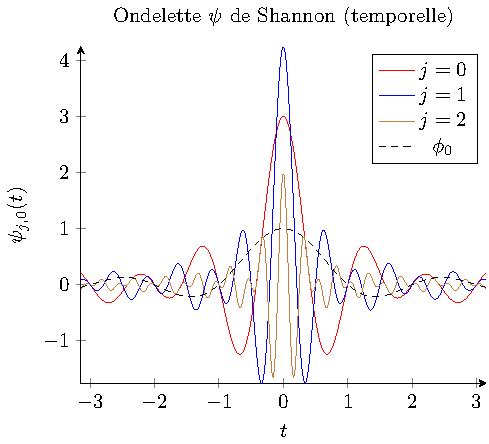
\includegraphics{Figs/shannon}}
	\label{fig:shannon}
	\floatbox[{\capbeside\thisfloatsetup{capbesideposition={right,bottom},capbesidewidth=4cm}}]{figure}[\FBwidth]
		{\caption{Des versions translatées $\psi_{j,k}$ des ondelettes $\psi_j$ du graphe précédent. Lorsque $j$ augmente, la fonction est parcourue plus rapidement d'un facteur $2^j$.}}
	{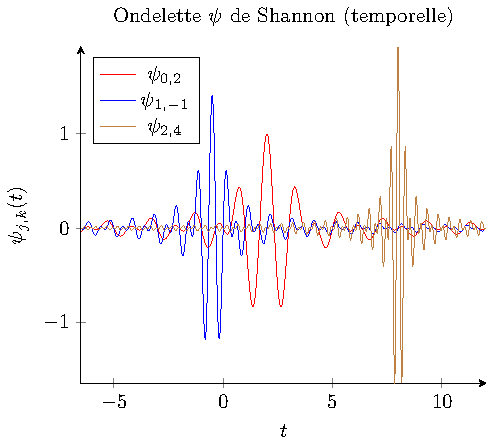
\includegraphics{Figs/shannonspat}}
\end{figure}
\begin{figure}
	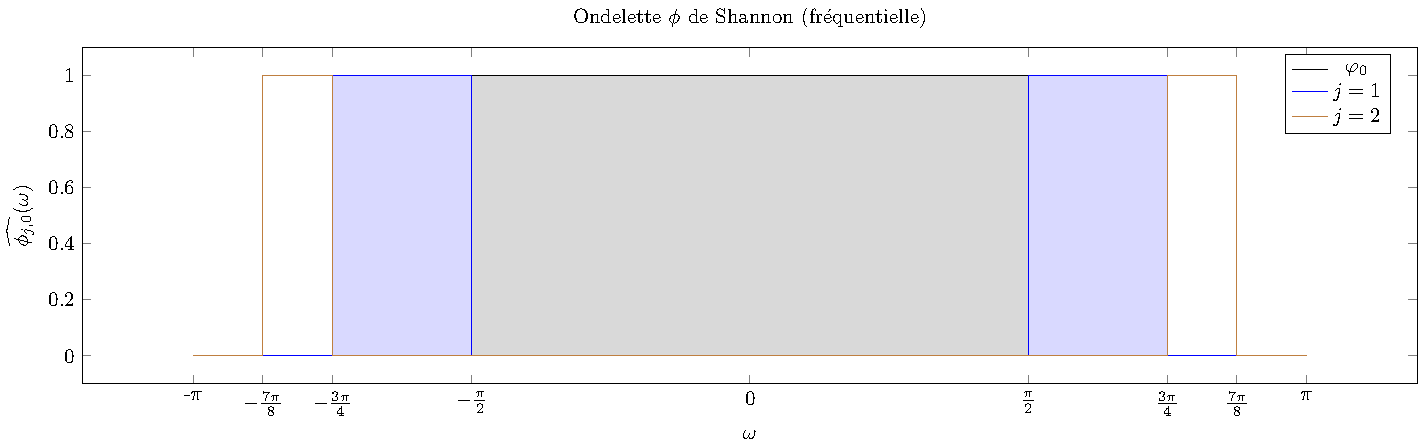
\includegraphics[width=17cm]{Figs/shannonfreq}
	\caption{La transformée de Fourier $\hat{\psi}$ de l'ondelette de Shannon $\Psi$. L'ondelette d'échelle $\phi_0$ est un filtre passe-bande $[-\frac{\pi}{2}, \frac{\pi}{2}]$, les ondelettes $ \psi_j$ sont des filtres passe bande qui recouvrent le reste de l'intervalle avec des supports disjoints de taille $2^{-j}$. On peut ainsi vérifier toutes les propriétés de l'analyse multi-résolution pour l'ondelette de Shannon sur les fonctions à bande limitée (c'est à dire, dont le support de la transformée de Fourier est borné).
	}
\end{figure}
\begin{remarque}
	Dans la définition des ondelettes $\psi_{j,k}$ engendrées par $\psi$, le coefficient $j$ correspond au facteur d'échelle\footnote{Du point de vue des notations, on considère que $j$ tend vers l'infini, signifie que $\psi_j$ analyse les hautes fréquences, ce choix de notation n'est pas uniforme dans la littérature, par exemple Stéphane Mallat et Ingrid Daubechies, utilisent $-j$ par rapport à nos notations. Par contre les notations utilisées correspondent à celles de Stéphane Jaffard et Yves Meyer. Mais cependant tous les résultats sont bien entendu équivalents.},
	en raison du facteur $2^j$ devant la variable, au fur et à mesure que $j$ augmente, l'ondelette est parcourue de plus en plus vite. Ainsi, augmenter $j$ revient à augmenter la fréquence de $\psi$, c'est à dire d'éloigner le support de $\hat{\psi}$ de l'origine. 
	Le coefficient $k$ correspond à une translation de l'ondelette $\psi_j$, en ce sens, l'analyse par ondelette, permet une analyse à la fois en temps (par rapport à $k$) et en fréquence (par rapport à $j$).
	\newline 
	En effet, de façon plus précise et formelle, on a par l'action de la transformée de Fourier sur les dilatations: 
	\begin{equation}
		\widehat{\psi_{j,0}}(\omega) = 2^{-\frac{j}{2}}\hat{\psi}(\frac{\omega}{2^j})
	\end{equation}
	et par l'action de la transformée de Fourier sur les translations:
	\begin{equation}
		\widehat{\psi_{j,k}}(\omega) = 2^{-\frac{j}{2}}\hat{\psi}(\frac{\omega}{2^j})e^{-2i\pi 2^{-j}k\omega}.
	\end{equation}
	On peut voir que l'analogie temps-fréquence dans le cadre des ondelettes implique en un certain sens le point de vue temps-fréquence de l'analyse Fourier.
	En effet, si on prend $\psi$ l'ondelette de Shannon (voir \ref{fig:shannon}), alors sa transformée de Fourier $\hat{\psi}$ est la fonction indicatrice sur $[-2\pi, \pi]\cup[\pi, 2\pi]$.
	Donc, à échelle $j$ fixée, on a que $\widehat{\psi_{j,k}}$ est supporté sur $B_j := [-2\pi2^{j+1}, -\pi2^j]\cup[\pi2^j, \pi2^{j+1}]$ et vaut:
	\begin{equation}
		\widehat{\psi_{j,k}}(\omega) = 2^{-\frac{j}{2}}e^{-2i\pi 2^{-j}k\omega}.
	\end{equation}
	Regardons maintenant la projection de $f\in L^2(\mathbb{R})$ sur les translatés de $\psi_j$, on a:
	\begin{equation}
		\langle f, \psi_{j,k} \rangle = \langle \hat{f}, \widehat{\psi_{j,k}} \rangle = \int_{B_j} \hat{f}(\omega) 2^{-\frac{j}{2}} e^{2i\pi2^{-j}k\omega} d\omega
	\end{equation}	
	donc en sommant par rapport à $k$ on a que la projection à $j$ fixé correspond à un développement en série de Fourier de $f$ avec les fréquences dans $B_j$.
	Donc l'intuition que lorsque $j$ augmente, la fréquence augmente, coincide exactement avec la notion de fréquence de la théorie de Fourier lorsque on considère l'ondelette de Shannon.

\end{remarque}
Donc étant donnée une famille d'ondelettes $\{\psi_{j,k}\}_{j,k \in \mathbb{Z}}$, comme on l'a vu on peut associer à une fonction $f\in L^2(\mathbb{R})$, ses coefficients d'ondelettes
\begin{equation}
	Wf = (\langle f, \psi_{j,k} \rangle )_{j,k \in \mathbb{Z}}
\end{equation}
et on se demande alors si à partir de ces coefficients on peut reconstruire $f$.
\begin{figure}[h]
	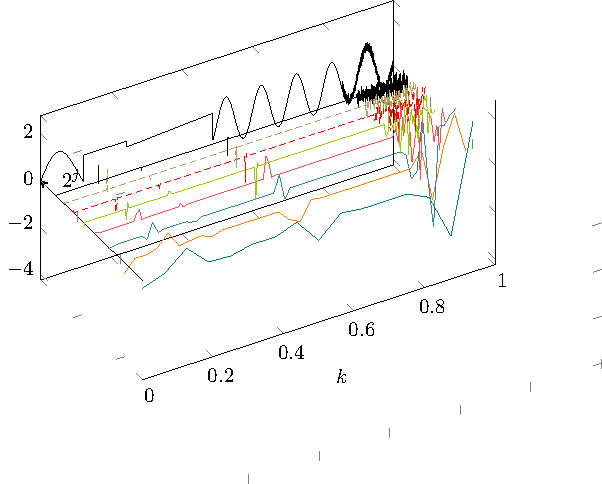
\includegraphics{Figs/wavelet}
	\caption{Les coefficients d'ondelette (pour l'ondelette de Daubechies D4) d'un signal présentant des zones de différentes régularité. Les coefficients les plus proches du signaux correspondent aux échelles les plus fines. On remarque que ces coefficients sont très petits dans les zones sans discontinuités. On peut voir que les hautes valeurs de ces coefficients (proches des discontinuités) se propagent vers les plus grandes échelles en s'étalant.}
\end{figure}
Cela revient ainsi à déterminer si la famille d'ondelettes est un frame d'ondelette. 
Ici on ne cherchera pas a énumérer et a vérifier des frames d'ondelettes, un très grand nombre de frames d'ondelettes existent\footnote{Pour une introduction au sujet des ondelettes par les frames on peut recommander le livre d'Ingrid Daubechies \cite{daubbook}, pour un théorème donnant une construction simple d'ondelettes en dimension $d\geq 1$ avec un échantillonage arbitraire (au lieu de l'échantillonage dyadique) on peut consulter \cite{IrregWav} et pour une liste d'ondelettes \url{https://en.wikipedia.org/wiki/Wavelet#List_of_wavelets}}, on admet ainsi l'existence des frames d'ondelettes. 
\newline
Supposons ainsi que l'on dispose d'un frame d'ondelettes et que ce frame est équilibré (c'est à dire que les bornes de frame $m$ et $M$ sont égales), alors on dispose d'une formule de reconstruction (d'après Daubechies 3.2.2)
\begin{equation}
	f = \frac{1}{M} \sum_{j,k} \langle f, \psi_{j,k}\rangle \psi_{j,k}.
\end{equation}
Cependant bien que la formule précédente permette une reconstruction elle suppose de parcourir des indices sur $\mathbb{Z}$ ce qui pourrait créer des complications concernant la convergence (d'un point de vue théorique ou pratique).
On va ici très rapidement introduire la notion d'analyse multi-échelle qui permet de simplifier la formule de reconstruction.
Construisons ici une analyse multi-échelle (ici de $L^2(\mathbb{R})$), considérons tout d'abord une suite d'espaces emboités satisfaisant 
\begin{equation*}
	\{0\}=	\lim_{j\to -\infty} \bigcap_{j}^{+\infty} V_i \subset \cdots \subset V_{-1} \subset V_0 \subset \cdots V_i \subset V_{i+1} \subset \cdots \subset \lim_{j\to \infty} \bigcup_{-\infty}^{j} V_i = L^2(\mathbb{R}).  
\end{equation*}
L'intérêt d'avoir une telle suite d'espaces emmboités est que étant donnée une fonction $f\in L^2(\mathbb{R})$, on peut considérer sa projection orthogonale dans un $V_i$, on a alors une approximation $f_i$ de $f$ dans $V_i$, si on souhaite améliorer l'approximation de $f$ il suffit alors de remonter dans ces espaces emboités pour avoir une reconstruction avec une précision arbitraire.
Introduisons maintenant la propriété qui va permettre de voir cette suite d'espaces comme une analyse multi-échelle
\begin{equation}
	f(\cdot) \in V_j \iff f(\frac{\cdot}{2^j}) \in V_0,
\end{equation}
c'est à dire que les fonctions d'un espace $V_j$ sont des versions dilatées d'un facteur $2^{-j}$ des fonctions de l'espace $W_0$.
Ajoutons maintenant la condition que $V_0$ contient toutes les translations entières de ses éléments, c'est à dire
\begin{equation}
	f \in V_0 \iff f(\cdot - n) \in V_0 \forall n \in \mathbb{Z}.
\end{equation}
Ainsi, une fonction qui appartient à $V_j$ s'écrit comme une combinaison linéaire de versions translatées et dilatées de fonctions appartenant à $V_0$.
De plus, quelque soit $j$ on peut prendre $W_j$ le complémentaire orthogonal de $V_j$ dans $V_{j+1}$, 
\begin{equation}
	f = \pi_{V_0}(f) +\sum_{i>0} \pi_{W_j}(f) 
\end{equation}
donc afin d'avoir une formule de reconstruction, il suffit de connaitre un frame de $V_0$ et de même pour chaque $W_j$. 
On peut maintenant revenir aux ondelettes, on considère que l'on connait $\varphi \in L^2(\mathbb{R})$ tel que $(\varphi_{k})_{k\in \mathbb{Z}}$, en notant $\varphi_k$ les translatés par $k$ de $\varphi$, soit une base de $V_0$ et $(\psi_{j,k})_{j\in \mathbb{N}^*, k \in \mathbb{Z}}$ un frame de l'orthogonal de $V_0$ dans $L^2(\mathbb{R})$, on pose alors $W_j = W_{j-1} \bigoplus Vect(\{\psi_{j,k}\}_{k\in \mathbb{Z}})$ et on obtient ainsi que l'analyse multi-échelle ainsi construite fournit une formule de reconstruction\footnote{Dans la formule de reconstruction les deux sommes sur $\mathbb{Z}$ ne sont pas problématiques car les fonctions considérées sont dans $L^2(\mathbb{R})$ donc avec une décroissance suffisament rapide, donc seulement un nombre fini de $\langle f, \varphi_{0,k} \rangle$ sont différents de 0 si $\varphi_0$ a une décroissance suffisament rapide (et de même pour chaque $\psi_j$).}
\begin{equation}
	f = \sum_{k\in \mathbb{Z}} \langle f, \varphi_{k} \rangle \varphi_{k} + \sum_{j = 1}^{+\infty} \sum_{k\in \mathbb{Z}} \langle f, \psi_{j,k} \rangle \psi_{j,k}.
\end{equation}
On appelle l'application $\varphi_0$ ondelette d'échelle.

\section{Décroissance des coefficients et régularité}
\subsection{Approximation linéaire et régularité}
On s'intéresse dans cette partie au lien entre une fonction $f\in L^2(]0, 1[)$ et son approximation dans une base. On verra un résultat reliant la décroissance des coefficients de la fonction dans une base fixée et la vitesse de convergence de la reconstruction. 
On verra ensuite à l'aide de ce résultat, que pour la base de Fourier (et resp. certaines bases d'ondelettes), on obtient des formules de reconstruction pour les fonctions dérivables (et resp. pour les fonctions Lipschitziennes) avec une erreur de reconstruction qui décroit rapidement.
\newline 
On considère ainsi un espace d'approximation de fonctions $U_N \subset L^2([0, 1])$.
Par construction, la meilleure approximation linéaire de $f$ dans $U_N$, est la projection orthogonale $f_N$ de $f$ dans $U_N$, qui peut être obtenue à l'aide de la base biorthogonale de synthèse associée $(\tilde{\phi}_k)_{k=1, \cdots, N}$ et la formule de reconstruction :
\begin{equation}
	f_N = \sum_{k=0}^{N-1}\langle f, \phi_k \rangle \tilde{\phi}_k.
\end{equation}
Afin de mesurer l'erreur d'approximation par rapport à $f$, on considère une base $\mathcal{B} = \{g_k\}_{k\in \mathbb{N}}$ de l'espace $L^2([0, 1])$ entier à laquelle on ajoute la condition de contenir une famille $(g_k)_{k\in I}$, avec $\#I = N$ qui forme une base de l'espace d'approximation $U_N$.
On peut ainsi écrire, en réordonnant la famille $(g_k)$,  $f_N \in U_N$ dans cette base :
\begin{equation}
	f_N = \sum_{k=0}^{N-1} \langle f, g_k \rangle g_k 
\end{equation}
et les $\{g_k\}_{\mathbb{N}}$ formant une base de $L^2([0, 1])$, on peut écrire $f$ dans cette base:
\begin{equation}
	f = \sum_{k=0}^{+\infty} \langle f, g_k \rangle g_k.
\end{equation}
On obtient donc que la partie orthogonale à la famille $\{\phi_k\}_{k=0, \cdots, N-1}$, est celle analysée par $\{g_k\}_{k\geq N}$.
C'est à dire, 
\begin{equation}
	f - f_N = \sum_{k=N}^{+\infty} \langle f, g_k \rangle g_k 
\end{equation}
et la mesure de l'erreur d'approximation avec $N$ coefficients est donc 
\begin{equation}
	\varepsilon_l(N, f) = ||f-f_N||^2 = \sum_{k=N}^{+\infty} |\langle f, g_k\rangle|^2.
\end{equation}
Comme on a supposé que $f\in L^2([0, 1])$ et que la famille $(g_k)$ est génératrice, on a que l'erreur d'approximation tend vers $0$ lorsque $N$ augmente.
On va maintenant s'intéresser au théorème suivant de Stéphane Mallat qui relie la décroissance des coefficients de $f$ dans la base de $L^2([0, 1])$ à la vitesse de décroissance de l'erreur d'approximation de la fonction.
\begin{theoreme}
	Soit $r > 1/2$, il existe des constantes $A, B > 0$ telles que si 
	\begin{equation}
		\sum_{k=0}^{+\infty} |k|^{2r}|\langle f, g_k \rangle |^2 < \infty,
	\end{equation}
	alors on a 
	\begin{equation}\label{eq:regframe}
		A \sum_{k=0}^{+\infty} k^{2r}|\langle f, g_k \rangle |^2 \leq 
		\sum_{N=0}^{+\infty} N^{2r-1} \varepsilon_l(N, f) \leq
		B \sum_{k=0}^{+\infty} k^{2r} |\langle f, g_k\rangle |^2
	\end{equation}
	et ainsi on a $\varepsilon_l(N, f) = o(N^{-2r})$.
\end{theoreme}
\begin{proof}
	On développe le terme au centre de l'égalité dela façon suivante 
	\begin{equation*}
		\sum_{N=0}^{\infty} N^{2r-1} \varepsilon_l(N, f) =
		\sum_{N=0}^{\infty} \sum_{k=N}^{\infty} N^{2r-1} |\langle f, g_k \rangle |^2 =
		\sum_{k=0}^{+\infty} |\langle f, g_k \rangle |^2 \sum_{N=0}^{k} N^{2r-1}.
	\end{equation*}
	Puis on majore des deux côtés avec 
	\begin{equation}
		\int_{0}^M x^{2r-1} dx \leq \sum_{N=0}^m N^{2r-1} \leq \int_{1}^{m+1} x^{2r-1}dx.
	\end{equation}
	En calculant les deux intégrales on déduit 
	\begin{equation}
		A m^{2r} \leq \sum_{N=0}^{m} N^{2r-1} \leq B m^{2r}
	\end{equation}
	où $A$ et $B$ dépendent seulement de $r$, ce qui nous donne \ref{eq:regframe}.
	Montrons maintenant $\varepsilon_l(N, f) = o(N^{-2r})$, remarquons tout d'abord que $\varepsilon_l(N, f)$ est décroissant par rapport à la première variable, on déduit de cela
	\begin{equation*}
		\varepsilon_l(N, f)\sum_{m=N/2}^{N-1} m^{2r-1} \leq \sum_{m=N/2}^{+\infty} m^{2r-1} \varepsilon_l(m, f)
	\end{equation*}
	on a donc avec le calcul précédent que le terme de droite converge quel que soit le choix de $N$, et ainsi
	\begin{equation*}
		\lim_{N \to +\infty} \sum_{m=N/2}^{+\infty} m^{2r-1}\varepsilon_l(m, f) = 0
	\end{equation*}
	donc tous les termes de l'inégalité précédente tendent vers 0. 
	De plus, $\sum_{m = N/2}^{N-1} m^{2r-1} \geq CN^{2r}$ et donc
	\begin{equation*}
		\lim_{N\to \infty} \varepsilon_l(N, f)N^{2r} = 0.
	\end{equation*}
\end{proof}
On a ainsi démontré que si $f$ appartient à l'espace
\begin{equation}
	W_{\mathcal{B}, r} =\{f : \sum_{m=0}^{+\infty} m^{2r} |\langle f, g_m \rangle |^2 < \infty\}
\end{equation}
alors l'approximation linéaire dans la base $\mathcal{B}$ décroit au moins comme $N^{-2r}$.
On montrera dans la prochaine sections que si $\mathcal{B}$ est une base de Fourier alors $W_{\mathcal{B}, r}$ contient les fonctions $r$-différentiables. 
On montrera ensuite que si $\mathcal{B}$ est une base d'ondelette avec une certaine propriété alors l'espace $W_{\mathcal{B}, r}$ contient les fonctions $\alpha$-Lipschitziennes pour $1 < \alpha < r$.
Des énoncés réciproques existent aussi et des démonstrations de ceux-ci peuvent être trouvés dans l'article de Stéphane Jaffard \cite{jaffard} ou bien dans le livre de Stéphane Mallat \cite{mallatbook}.
\subsection{Décroissance des coefficients de Fourier}
On considère ici $\mathcal{B} = (e_{n})_{n \in \mathbb{Z}}$ la base de Fourier ( voir 1.3.3) de $L^2(\mathbb{R})$.
On peut ainsi définir l'espace $U_N = \{f \in L^2(\mathbb{R}) : |k| > N \implies \hat{f}(k) = 0\}$ sur lequel $\mathcal{B}_N = (e_{n})_{|n|\leq N}$ est une base. 
Avec des mots, $U_N$ est l'espace des fonctions qui ne sont portées par aucune exponentielle complexe de fréquence supérieure ou égale à $N$.
Le théorème de Shannon nous indique que $2N$ fréquences permettent de séparer n'importe laquelle de ces fonctions, ainsi on  a la formule de reconstruction.
On dispose ainsi d'une formule de projection (et de reconstruction), soit $f \in L^2(\mathbb{R})$
\begin{equation}
	f_N(t) = \sum_{|n|\leq N/2} \langle f, e_n \rangle e_n(t) \in U_N.
\end{equation}
Ainsi $f_N$ est une approximation linéaire de $f$, et $f$ sera rapidement approximée si $f$ n'a pas trop de hautes fréquences. 
Montrons maintenant que la vitesse de décroissance des coefficients de Fourier est liée à la régularité de la fonction.
Tout d'abord, revenons à $L^2(\mathbb{R})$ considérons que $f$ est dérivable, alors on a en intégrant par parties
\begin{equation}
	\hat{f}'(\omega)\int_{-\infty}^{+\infty} f'(t) e^{i \omega t} dt = i \omega \int_{-\infty}^{+\infty} f(t) e^{i\omega t} dt = i \omega \hat{f}(\omega) 
\end{equation}
et en utilisant la formule de Plancherel on a 
\begin{equation}
	||\hat{f}'||_2^2 = \int_{-\infty}^{+\infty} |\omega|^2 |\hat{f}(\omega)|^2 d\omega = \int_{-\infty}^{+\infty} |f'(t)|^2 dt = ||f'||_2^2.
\end{equation}
On est ainsi amenés à définir une régularité dans $L^2(\mathbb{R})$, distincte de la dérivabilité en un point avec la définition suivante :
\begin{definition}
	On dit que $f\in L^2(\mathbb{R})$ est différentiable au sens de Sobolev si
	\begin{equation*}
		\int_{-\infty}^{+\infty} |\omega|^2|\hat{f}(\omega)|^2 d\omega < \infty. 
	\end{equation*}
\end{definition}
Et avec cette définition on peut définir pour n'importe quel $r>0$ l'espace des fonction $r$-différentiables de Sobolev:
\begin{equation}
	W^r(\mathbb{R}) =\{ f \in L^2(\mathbb{R}) : \int_{\mathbb{R}} |\omega|^{2r} |\hat{f}(\omega)|^2 d\omega < \infty \}.
\end{equation}
Ainsi d'après le théorème sur la vitesse d'approximation de Mallat, l'approximation linéaire dans la base de Fourier d'une application $r$-différentiable décroit plus vite que $N^{-2r}$.
\subsection{Décroissance des coefficients d'ondelettes}
On va montrer dans cette section que en imposant certaines conditions sur les ondelettes, alors il est possible de démontrer que la régularité au sens de Lipschitz, implique une décroissance des coefficients d'ondelettes.
On pourra ensuite relier cette décroissance aux discussions de la fin de la partie précédente.
\newline
Tout d'abord posons les définitions dont nous aurons besoin dans cette partie,
\begin{definition}
	Soit $\alpha$ tel qu'il existe un entier strictement positif $r$ tel que $r-1 \leq \alpha <r$. On dit qu'une fonction $f$ est $\alpha$-Lipschitz en $t_0$ si il existe une constante $C>0$ et un polynôme $P_{t_0}$ de degré strictement inférieur à $r$, tels que pour tout $t$ qui appartient à un voisinage $T_0$ de $t_0$, on a 
	\begin{equation*}
		|f(t) - P_{t_0}(t)| \leq C|t-t_0|^{\alpha}
	\end{equation*}
\end{definition}
Avec cette définition on vérifie immédiatement que si on considère un signal $r$-dérivable au sens classique, alors en utilisant l'approximation avec un polynôme de Taylor du signal, on a pour tout $0 < \alpha \leq r$, que le signal est partout $\alpha$-Lipschitz.
\newline
On peut facilement relier cette définition avec les ondelettes, en considérant les moments d'ondelette.
On considère ainsi $\{\psi_{j, k} = \psi( 2^{\frac{j}{2}}\psi(2^j\cdot -k)\}_{j,k}$ une base orthonormale d'ondelettes de $L^2([0, 1])$, et on a le coefficient d'ondelette à l'échelle $j$ et à l'instant $k$ donnée par
\begin{equation*}\label{eq:defWx}
	Wf (j, k) = \langle f, \psi_{j,k} \rangle = \int f(t) \psi_{j,k}(t)dt.
\end{equation*}
\begin{remarque}
Remarquons ici que l'on peut exprimer cette projection à partir de l'ondelette prise à l'instant $0$
\begin{equation*}
	\widecheck{\psi_j}(t) = \psi_{j, 0}(-t) = \psi(-2^jt),
\end{equation*}
et ainsi en faisant un changement de variable dans \ref{eq:defWx}, on obtient
\begin{equation}
	Wf(j,k) = f \star \widecheck{\psi_j}(k).
\end{equation}
On peut ainsi interpreter le coefficient d'ondelette pris en $(j,k)$ comme la corrélation entre le signal pris en $k$ avec une ondelette à l'échelle $j$.
C'est à dire qu'un coefficient avec une grande valeur indique une grande similitude entre l'ondelette et le signal (l'ondelette approxime bien le signal) alors qu'un petit coefficient indique que l'ondelette et le signal ont peu en commun\footnote{L'ondelette et le signal ont peu en commun au sens où ils sont de façon équivalente, presque orthogonaux, et donc ce coefficient à un poids faible dans la formule de reconstruction.}.
\end{remarque}
Rappelons aussi qu'un condition nécessaire pour que $\psi$ soit une ondelette génératrice est
\begin{equation*}
	\int \psi (t)dt = 0.
\end{equation*}
\begin{definition}
	Soit $m$ un entier strictement positif.
	On dit que $\psi$ a $m$-moments nuls si
	\begin{equation*}
		\int t^k \psi(t)dt = 0 \quad, \forall k < m.
	\end{equation*}
\end{definition}
De cette définition on déduit que si $P$ est un polynôme de degré strictement inférieur à $m$ et si l'ondelette a $m$-moments nuls, alors
\begin{equation}\label{eq:momPol}
	\int \psi(t) p(t) dt = 0.
\end{equation}
Ainsi si $f(t) = P(t) +\epsilon$ où $\epsilon$ représente un bruit, on a 
\begin{equation*}
	\langle f, \psi_{j,k} \rangle = o(\epsilon)
\end{equation*}
ainsi les coefficients de l'ondelette d'échelle suffisent à reconstruire $f$.
C'est ainsi que si on considère une ondelette avec un certain nombre de moments nuls, alors dans les parties régulières du signal, les coefficient d'ondelettes seront petits, alors que dans les zones avec des irrégularités ou des discontinuités, les coefficients resteront grands.
On peut aussi remarquer que si les irrégularités sont séparées, alors en affinant l'échelle d'analyse, le support des ondelettes diminue et alors de moins en moins de coefficients auront une valeur importante, ainsi les seuls coefficients qui resteront grand en changeant d'échelle sont ceux qui contiennent une zone irrégulière. 
\newline
On va maintenant démontrer le théorème suivant de Jaffard qui permet de préciser cela,
\begin{theoreme}\label{th:Jaffard}
	Si $f$ est $\alpha$-Lipschitz en $t_0$ avec $0 < \alpha \leq m$ où $m$ est un entier.
	Alors, il existe une constante $C >0$ telle que 
	\begin{equation*}
		|Wf(j, k)| \leq C2^{-j(\alpha + \frac{1}{2})}(1 + |2^{-j}t - t_0|2^{j\alpha}).
	\end{equation*}
\end{theoreme}
\begin{proof}
	Remarquons tout d'abord que, soit $P$ un polynôme de degré strictement inférieur à $m$, et $\psi$ une ondelette a $m$-moments nuls, alors, par changement de variable et d'après \ref{eq:momPol} on a :
	\begin{equation}\label{eq:polAnn}
		WP(j, k) = \int 2^{j/2} \psi(2^jt - 2^{-j}k) P(t)dt 
		= \int 2^{j/2}\psi(t')P(2^jt' - 2^{-j} k) 2^{-j} dt' = 0.
	\end{equation}
	Par hypothèse, $x$ est $\alpha$-Lipschitz en $t_0$, donc il existe $P_{t_0}$ un polynôme de degré inférieur à $m$ tel que $|f(t) - P_{t_0}(t)| \leq C|t - t_0|^{\alpha}$.
	En utilisant la linéarité de l'intégrale et en appliquant une inégalité triangulaire on obtient
	\begin{align*}
		|Wf(j,k)| &= \left|\int (f(t) -P_{t_0}(t) + P_{t_0}(t)) \psi_{j, k}(t) dt\right| \\
			&\leq \left|\int (f(t) - P_{(t_0}(t)) \psi_{j,k}(t)dt\right| + \left|\int P_{t_0}(t) \psi_{j,k}(t)dt\right| \\ 
			&\leq \int| f(t) - P_{t_0}(t)| |\psi_{j,k}(t)|dt  
	\end{align*}
	la dernière inégalité étant obtenue en utilisant \ref{eq:polAnn} sur le terme de droite et en faisant entrer la valeur absolue dans la première intégrale.
	On utilise maintenant le fait que $f$ est $\alpha$-Lipschitz et on fait un changement de variable, on obtient ainsi
	\begin{align*}
		| Wf(j,k)| \leq \int |f(t) - P_{t_0}(t)||\psi_{j,k}(t)|dt &\leq C\int |t - t_0|^\alpha 2^{j/2} |\psi(2^jt - k)|dt \\
		&\leq C \int |2^{-j} t' + 2^{-j}k - t_0|^\alpha 2^{-j/2} |\psi(t')| dt'. 
	\end{align*}
	Pour obtenir l'inégalité suivante on utilise
	\begin{equation*}
		|a + b|^\alpha \leq |2*\max(|a|, |b|)|^\alpha \leq 2^\alpha (|a|^\alpha + |b|^\alpha)
	\end{equation*}
	et on a ainsi
	\begin{align*}
		|Wf(j,k)| &\leq 2^\alpha C \int (|2^{-j}t'|^\alpha + |2^{-j}k-t_0|^\alpha)2^{-j/2} |\psi(t')|dt'\\
		&\leq 2^\alpha C 2^{-j(\alpha + 1/2)}\left( \int|t'|^\alpha |\psi(t')|dt' + |2^{-j}k-t_0|^\alpha 2^{\alpha j}\int |\psi(t')|dt' \right)
	\end{align*}
	Ce qui donne le résultat dès que les intégrales considérées sont définies, ce qui est le cas par exemple si l'ondelette est à support compact ou bien à décroissance suffisamment rapide. 
\end{proof}
On peut combiner le théorème de Jaffard avec une analyse multi-échelle d'ondelettes avec la proposition suivante :
\begin{proposition}
	Soit $f:]0,1[ \to \mathbb{R}$ une fonction $\alpha$-Lispchitzienne avec $\alpha>1$, alors il existe une constante $C>0$ et une base d'ondelette orthonormales associée à une multiresolution $\{(\psi_{j,k})_{(i,j): j\geq J, 2^{j} > k\geq 0}\}, \{\varphi_{J,k}\}_k$ avec $m>\alpha$ moments nuls telle que  
	\begin{equation}
		\varepsilon_l(f, 2^J) = ||f - \sum_{k=0}^{2^J -1} \langle f, \varphi_{J,k}\rangle \tilde{\varphi}_{J,k}||_2^2 \leq C 2^{-2J\alpha} = CN^{-2\alpha}
	\end{equation}
	avec $N=2^J$.
\end{proposition}
\begin{proof}
	L'existence d'une telle base d'ondelette n'est pas démontrée ici, des constructions peuvent être trouvées dans (ajouter ref) pour obtenir des bases de $L^2(\mathbb{R})$, on peut ainsi considérer une telle multirésolution donnée par une ondelette de Daubechies ou bien une coiflet à $m>\alpha$ moments nuls.
	Il est ensuite possible, avec quelques difficultés d'obtenir depuis ces ondelettes, une base orthonormale de $L^2(]0,1[)$ (ajouter ref).
	Soit $f$ une fonction $\alpha$-Lipschitzienne sur $]0,1[$, on a ainsi d'après la partie sur les frames et l'existence de la base d'ondelette précédente admise, une formule de reconstruction
	\begin{equation*}
		f = \sum_{k=0}^{2^J -1} \langle f, \varphi_{J,k}\rangle \tilde{\varphi}_{J,k} + \sum_{j=J+1}^{+\infty}\sum_{k=0}^{2^j-1} \langle f, \psi_{j,k} \rangle \tilde{\psi}_{j,k}. 
	\end{equation*}
	On a ainsi, en réécrivant l'équation et en prenant la norme
	\begin{equation*}
		\varepsilon(f, 2^J) = ||f - \sum_{k=0}^{2^J -1} \langle f, \varphi_{J,k}\rangle \tilde{\varphi}_{J,k}||_2^2 =|| \sum_{j=J+1}^{+\infty}\sum_{k=0}^{2^j-1} \langle f, \psi_{j,k} \rangle \tilde{\psi}_{j,k}||_2^2. 
	\end{equation*}
	On peut alors majorer le terme de droite en utilisant le fait que la famille d'analyse est génératrice, on obtient
	\begin{equation*}
		\varepsilon(f, 2^J) \leq \sum_{j=J+1}^{+\infty} ||\sum_{k=0}^{2^j -1} \langle f, \psi_{j,k} \rangle \tilde{\psi}_{j,k} ||_2^2
	\end{equation*}
	et en utilisant le fait que les ondelettes sont normalisées on a
	\begin{equation*}
		\varepsilon(f, 2^J) \leq \sum_{j=J+1}^{+\infty} \sum_{k=0}^{2^j -1} |\langle f, \psi_{j,k} \rangle|^2
	\end{equation*}
	on utilise maintenant le théorème \ref{th:Jaffard} et on obtient\footnote{Le théorème de Jaffard est pour une fonction ponctuellement Lipschitzienne, on considère ici une fonction $\alpha$-Lipschitzienne en tout point, donc le terme en $(1 + \frac{|2^{-j}k -t_0|}{2^j})$ n'apparait pas.}
	\begin{align*}
		\varepsilon(f, 2^J) &\leq \sum_{j=J+1}^{+\infty} \sum_{k=0}^{2^j -1} C^2 2^{-j(2\alpha + 1)} \\
		&\leq \sum_{j=J+1}^{+\infty} C^2 2^{-j(2\alpha + 1)} 2^{j} = \sum_{j=J+1}^{+\infty} C^2 2^{-j2\alpha} \\
		&\leq \frac{C^2}{1 - 4^{-\alpha}} 2^{-2J\alpha}	
	\end{align*}
	ce qui prouve la proposition.
\end{proof}



\chapter{Reconstruction parcimonieuse et $||\cdot||_1$}
\section{Introduction à (P0)}
Dans ce qui précède, nous nous sommes intéressés aux propriétés qui font qu'une famille de vecteurs permet de reconstruire une famillle de signaux.
Nous avons vu différentes bases (Fourier et ondelettes) et nous avons vu que ces bases permettent de reconstruire des signaux présentant un certain type de régularité avec des coefficients qui suivent une décroissance assez rapide.
\newline
On a par exemple vu que l'on pouvait reconstruire les fonctions Lipschitziennes avec une bonne précision en utilisant une base d'ondelettes orthonormale avec un certain nombre de moments nuls.
De plus, on a remarqué que si la fonction se comporte comme un polynôme d'un degré inférieur au nombre de moments nuls au voisinage d'un point, alors les coefficients d'ondelettes dans ce voisinage seront nuls.
De même, les seuls coefficients d'ondelette qui seront grands seront ceux au voisinage d'un point où aucune approximation par un polynôme de petit degré n'est efficace\footnote{Une analyse du théorème de Jaffard \ref{th:Jaffard} montre que les coefficients affectés par une discontinuité forment un cône dans les coefficients d'ondelette autour du point de discontinuité. Ce cône se visualise dans la représentation temps-fréquence des coefficients d'ondelette, il part du point de discontinuité et s'élargit en diminuant le coefficient d'échelle $j$. La largeur de ce cône dépend de la régularité $\alpha$ de la fonction.}.
Ainsi, la représentation avec ces ondelettes d'une fonction ne possédant que quelques points où elle est irrégulière sera approximée avec peu de coefficients.
L'intérêt de cela est que de façon naive, afin de déterminer une fonction, il faut connaitre sa valeur en chaque point (sa valuation), ainsi, si l'on souhaite faire un traitement par ordinateur de cette fonction, il faut stocker chacun des points de la fonction.
Avec ce que l'on a fait, on sait qu'en fait on peut reconstruire la fonction avec un plus petit nombre de coefficients que la fonction n'a de points.
En ce sens, la représentation en ondelettes d'une fonction Lipschitzienne est parcimonieuse (peu de coefficients non nuls), alors que la représentation par la valuation d'une fonction Hölderienne n'est pas parcimonieuse.
\newline
Nous allons maintenant nous intéresser à l'autre direction de ce problème, c'est à dire que nous allons supposer que l'on dispose d'une famille de vecteurs et que la fonction que l'on cherche à reconstruire est une somme parcimonieuse de vecteurs de cette famille.
Cependant on connait seulement la valuation de cette fonction et pas les vecteurs sous-jacents qui permettent de représenter la fonction de façon parcimonieuse.
Aussi, on n'a pas supposé que cette famille est libre donc il n'y a pas une unique façon d'obtenir cette solution, en fait il y a une infinité de solutions dès que la famille n'est pas libre.
On va voir cependant que l'hypothèse de parcimonie est cruciale et qu'elle nous permettra de récupérer exactement les coefficients qui permettent l'écriture parcimonieuse de cette fonction.
\newline
Avant de poursuivre, il est important de remarquer que résoudre un tel problème requiert à priori de choisir la bonne décomposition parmi toutes les colonnes possibles qui est un problème combinatoire très difficile.
On va voir que pour exploiter la parcimonie on utilisera de façon répétitive la norme $||\cdot||_1$ pour trouver la solution parcimonieuse, contrairement au chapitre précédent dans lequel la norme $||\cdot||_2$ était omniprésente.
On peut donner une intuition géométrique à la préférence de la norme 1 par rapport à la norme 2 pour résoudre un problème ayant un lien avec la parcimonie.
On verra que ce que l'on cherche à résoudre est une équation du type $y=Fx$, donc pour trouver la solution minimale pour une certaine norme, il suffit de prendre la boule centrée en 0 de plus petit rayon avec la norme correspondante et la solution minimale revient à trouver l'intersection entre cette boule et le plan des solutions de $y=Fx$.


On peut donc représenter cela avec la figure \ref{fig:compball}, la boule unité pour la norme $||\cdot||_0$ correspondant aux axes (privés de l'origine), il est clair que la plupart des équation du type $y=Fx$ auront leur solution en norme 1 qui coincide avec celle en norme 0.
Par contre, un tel phénomène n'est pas vérifié pour la norme euclidienne.
	\begin{figure}[h]\label{fig:compball}
		\floatbox[{\capbeside\thisfloatsetup{capbesideposition={left,top},capbesidewidth=4cm}}]{figure}[\FBwidth]
		{\caption{Minimisation de $y=Fx$ pour la norme $\ell^1$. La solution de \ref{P1} est généralement celle de \ref{P0} sauf si les solutions sont parallèles à l'une des faces de la boule de $\ell^1$.}}
		{\includegraphics{Figs/l1vs1}}

		\floatbox[{\capbeside\thisfloatsetup{capbesideposition={right,bottom},capbesidewidth=4cm}}]{figure}[\FBwidth]
		{\caption{Minimisation de $y=Fx$ pour la norme $\ell^2$. La solution de \ref{P2} n'est généralement pas celle de \ref{P0} sauf si les solutions sont parallèles à l'un des axes.}}
		{\includegraphics{Figs/l1vs2}}
	
	\end{figure}


\section{Résolution de (P0)}
Formalisons maintenant ce que nous avons dit ci-dessus. 
On considère $\mathcal{F}$ un espace vectoriel et utilisons un dictionnaire $\Phi = \Phi_1 \cup \cdots \cup \Phi_D$ de bases, où chaque $\Phi_d$ est une base de $\mathcal{F}$. 
Ainsi $\Phi$ est une concaténation de bases\footnote{Ainsi $\Phi$ définit un frame.} et on s'intéresse aux façon d'écrire un signal $f\in \mathcal{F}$ dans $\Phi$, c'est à dire aux façon d'écrire
\begin{equation}\label{eq:defSSum}
	f = \sum_\gamma c_\gamma \phi_\gamma
\end{equation}
où l'indice $\gamma = (d, i)$ indique le dictionnaire $\Phi_d$ correspondant ainsi que le vecteur $\phi_{d, i} \in \Phi_d$.
On peut aussi écrire \ref{eq:defSSum} sous forme matricielle en posant $F_\Phi$ la matrice ayant pour lignes les vecteurs $\phi_\gamma$ et en posant $x = (c_\gamma)_\gamma$, on utilisera aussi la notation $x = (x_d)_{d=1, \cdots, D}$
On s'intéresse ainsi aux solutions de 
\begin{equation}
	f = F_\Phi x.
\end{equation}
Comme discuté précedemment, le choix des coefficients $c_\gamma$ n'est pas unique dès que $D>1$, cependant notre objectif n'est pas simplement de reconstruire $f$ (car n'importe quelle base $\Phi_i$ permet déjà cela), mais de trouver l'écriture de $f$ avec le minimum de coefficients non nuls.
Ainsi, le problème que l'on cherche à résoudre est 
\begin{equation}\label{P0}\tag{P0}
	\min ||x||_0\quad \text{tel que } f = F_\Phi x,
\end{equation}
où $||x||_0 = |\{\gamma : c_\gamma \neq 0\}|$ est le nombre de coefficients non nuls de $x$.
Cependant, la résolution en toute généralité de ce problème n'est pas faisable, en effet résoudre ce problème nécessite de résoudre \ref{P0} pour chaque combinaison de vecteurs du dictionnaire si $x$ est dans l'image.
Ainsi, le nombre de combinaisons possibles parmi tous les vecteurs croit bien trop vite pour permettre la résolution de \ref{P0} de cette façon, nous verrons donc comment résoudre ce problème en utilisant une autre méthode.
\newline
Il est important de noter qu'à ce stade il n'y a aucune raison de supposer que chercher une unique solution à (P0) a un sens.
En effet, quand on a choisi le dictionnaire $\Phi$ rien ne nous interdisait de prendre à chaque fois la même base et on aurait ainsi $D$ solutions identiques, ayant chacune la même parcimonie.
On a ainsi $D$ solutions, et si on prend une paire de solutions $x_1, x_2$, alors $F_\Phi(x_1 - x_2) = 0$, d'où on obtient qu'à n'importe laquelle des $D$ solutions, on peut ajouter, par exemple $x_1 - x_2$, et on obtient une nouvelle solution. 
Cependant, cette solution ne sera jamais moins parcimonieuse que l'une des $D$ solutions initiales.
Il est donc clair qu'il est nécessaire d'imposer des conditions sur les bases qui constituent le dictionnaire si l'on souhaite obtenir une solution unique.
Afin d'étudier cela commençons par un cadre simple dans lequel résoudre $P_0$ a un sens.
\begin{exemple}
	On étudie les signaux dans $\mathbb{R}^N$ et on choisi un dictionnaire constitué de la concaténation de la base de Fourier $ W = \{e_k(t) = \frac{1}{\sqrt{N}} e^{\frac{i 2\pi k t}{N}}\}_{0 \leq k \leq N -1}$ et de la base canonique de Dirac\footnote{Chaque vecteur de cette base vérifie $\delta_{k,i} = 1$ si $i = k$ et 0 sinon.} $T = \{\delta_k\}_{0 \leq k \leq N-1}$.
	Ainsi, avec ce choix $F_W$ est la matrice de Fourier discrète normalisée et $F_T$ est la matrice identité de taille $N$.
	Avec le théorème suivant, on va obtenir un principe d'incertitude, qui nous garantira qu'un signal ne peut pas être parcimonieux à la fois dans la base de Dirac, et dans la base de Fourier.
	\begin{theoreme}\label{th:Incert1}
		Soit un signal $f\in \mathbb{R^N}$ non nul, alors
		\begin{equation}
			||F_W f||_0 ||F_T f||_0 \geq N 	
		\end{equation}
		et ainsi
		\begin{equation}
			||F_W f||_0 + ||F_T f||_0 \geq 2 \sqrt{N}. 	
		\end{equation}
	\end{theoreme}
	\begin{proof}
		La preuve qui est faite ici est standard, on peut par exemple la trouver dans l'article \cite{taoprime}, on précise cependant la matrice $F_T$ qui permettra d'obtenir des généralisations directes par la suite.
		Soit $0 \leq \omega \leq N-1$ un entier, alors 
		\begin{align}
			|F_W(\omega)| &= |\hat{f}(\omega)| = \frac{1}{\sqrt{N}}|\sum_t f(t)e_\omega(t)| \\
				&\leq \frac{1}{\sqrt{N}}\sum_t |f(t)|,
		\end{align}
		d'où $\sup_\omega |F_W(\omega)| \leq \frac{1}{\sqrt{N}} \sum_t |f(t)|$.
		On pose maintenant $sign(f) = (\frac{f(t)}{|f(t)|})_t$ pour tous les $t$ tels que $f(t) \neq 0$ et 0 si $f(t) = 0$ et on a ainsi $\langle sign(f), sign(f) \rangle = ||F_T f||_0$, on va ainsi pouvoir montrer le théorème en utilisant successivement l'inégalité de Cauchy-Schwarz puis l'égalité de Parseval,
		\begin{align}
			\sup_\omega|F_W(\omega)| &\leq \frac{1}{\sqrt{N}}\sum_t |F_Tf (t)| = \frac{1}{\sqrt{N}}\langle sign(f), |f| \rangle \\
			&\leq  \frac{1}{\sqrt{N}} ||F_T||_0^{\frac{1}{2}} \langle |f|, |f| \rangle ^{\frac{1}{2}} =  \frac{1}{\sqrt{N}} ||F_T||_0^{\frac{1}{2}} \langle |F_W f|, |F_Wf| \rangle ^{\frac{1}{2}} \\
			&\leq   \frac{1}{\sqrt{N}} ||F_T||_0^{\frac{1}{2}} \langle |F_Wf|, |F_Wf| \rangle ^{\frac{1}{2}} =  \frac{1}{\sqrt{N}} ||F_T||_0^{\frac{1}{2}} \left( \sum_\omega|\hat{f}(\omega)|^2 \right)^{\frac{1}{2}}\\ 
			&\leq \frac{1}{\sqrt{N}}||F_T||_0^{\frac{1}{2}} ||F_W f||_0^{\frac{1}{2}} \sup_\omega |F_W(\omega)|.
		\end{align}
		On a ainsi montré la première partie du théorème, la deuxième partie provient directement de l'inégalité entre la moyenne arithmétique et la moyenne géométrique.
		En effet, on a 
		\begin{equation}
			\sqrt{||F_T f||_0 ||F_W f||_0} \leq \frac{||F_T f||_0 + ||F_W f||_0}{2}
		\end{equation}
	et on a déjà montré que le terme de gauche est supérieur ou égal à $\sqrt{N}$.
	\end{proof}
	Mentionnons que sans restrictions sur $N$, l'inégalité obtenue ne peut pas être améliorée, comme observé dans \cite{donohostark} \cite{DonohoHuo}, si $N$ est un carré, alors, la fonction avec des 1 seulement aux coefficients multiples de $\sqrt{N}$ et 0 ailleurs est sa propre transformée de Fourier.
	Elle a alors 2 écritures avec chacune $\sqrt{N}$ coefficients dans le dictionnaire $(T,W)$ et ainsi l'inégalité est atteinte.
	Une conséquence de cela est qu'une condition sur la parcimonie de la forme $||F_T f||_0 + ||F_W||_0 < K$ avec $K>\sqrt{N}$ ne pourra pas garantir l'unicité de la solution de (P0).
	Montrons que si $K = \sqrt{N}$ alors on a l'unicité de la solution de (P0).
	\begin{theoreme}\label{th:Incert2}
		Soit $N$ un entier positif, $(T,W)$ le dictionnaire Fourier-Dirac et un signal $f \in \mathbb{R}^N$, alors n'importe quel $x$ vérifiant $f = F_\Phi x = F_W x_W + F_T x_T$ et 
		\begin{equation}\label{eq:Incert1}
			||x_W||_0 + ||x_T||_0 < \sqrt{N}
		\end{equation}
		est l'unique solution de (P0).
	\end{theoreme}
	Supposons que pour $f$ donné non nul et supposons que l'on ait deux solutions de (P0), $x_1$ et $x_2$, ainsi $f = F_\Phi x_1, f = F_\Phi x_2$ et on a aussi $||x_1||_0 < \sqrt{N}, ||x_2||_0 < \sqrt{N}$.
	On a par linéarité de l'opérateur $F_\Phi$, 
	\begin{equation}
		F_\Phi( x_1 - x_2) = 0.
	\end{equation}
	Etudions ainsi les éléments du noyau de $F_\Phi$, posons $\mathcal{N} = \{\delta : F_\Phi \delta = 0\}$, et pour tout $\delta \in \mathcal{N}$, écrivons $\delta = (\delta_T, \delta_W)$, on a
	\begin{equation}
		F_T \delta_T + F_W \delta_W = 0
	\end{equation}
	ainsi, en utlilisant que les colonnes de $F_W$ forment une base, donc $F_W$ est une matrice orthogonale, on a 
	\begin{equation}\label{eq:structN}
		\delta_W = -F_W^t F_T \delta_T .
	\end{equation}
	On a donc montré que les éléments de $\mathcal{N}$ sont de la forme $\delta = (\delta_T, -F_W^t F_T \delta_T)$ et d'après le théorème \ref{th:Incert1}, on a que $\delta$ a au moins $2\sqrt{N}$ coefficients non nuls si $\delta$ est non nul. 
	En revenant a la situation initiale $\delta = x_1 - x_2$, on a une contradiction car à la fois $x_1$ et $x_2$ ont chacun moins de $\sqrt{N}$ coefficients, donc $\delta = 0$.
	Ainsi, si une solution existe avec moins de $\sqrt{N}$ coefficients, alors c'est la solution de (P0) et elle est unique.
	\newline
	Cependant, en choisissant $N = p$, où $p$ est un nombre premier\footnote{L'hypothèse $p$ premier est essentielle, la preuve reposant sur la non-existence de sous-groupes propres du groupe cyclique $\mathbb{Z}/p\mathbb{Z}$}, Terence Tao \cite{taoprime} a montré que l'on obtient l'inégalité
	\begin{equation}
		||F_T f||_0 + ||F_W f||_0 \geq p + 1
	\end{equation}
	et que l'inégalité est atteinte\footnote{L'inégalité est atteinte en ce sens qu'il existe $A\subset T$ et $B\subset W$ tels que $|A| + |B| = p+1$ et il existe une fonction $f$ telle que $Supp F_T f = A$ et $Supp F_W f = B$}.
	Grâce à ce principe d'incertitude plus fort que \ref{th:Incert1}, on obtient avec le même type de preuve\footnote{Voir \cite{CRT} pour les détails, un lemme sur l'injectivité d'un opérateur similaire $F_W$ est tout de même nécessaire pour conclure la preuve.} le résultat suivant
	\begin{theoreme}
		Soit $p$ un nombre premier et un signal $f \in \mathbb{R}^N$, alors n'importe quel $x$ vérifiant $f = F_\Phi x = F_W x_W + F_T x_T$ et
		\begin{equation}\label{eq:Incert2}
		||x_T||_0 \leq \frac{p}{2}
		\end{equation}
		est l'unique solution de \ref{P0}.
	\end{theoreme}
	On a ainsi vu qu'avec un dictionnaire constitué de Fourier et de Dirac la solution de \ref{P0} est unique, on a également vu brièvement, qu'en renforçant le principe d'incertitude sur les deux familles, alors on peut certifier qu'on a bien obtenu \it{la} solution de \ref{P0} pour des signaux avec un support plus grand.
\end{exemple}

\section{Résolution de (P1)}
On a ainsi vu dans la section précedente que le problème \ref{P0} de minimisation de la solution par rapport à la parcimonie admet une solution unique dès qu'une solution existe et que cette solution vérifie une condition de la forme \ref{eq:Incert1} ou \ref{eq:Incert2}.
Cependant, on a aussi vu au début de la section précédente que le problème \ref{P0} est un problème de nature combinatoire et le nombre de combinaisons possibles augmentant très vite par rapport à $N$, sa résolution n'est pas faisable et ainsi il est nécessaire d'avoir une autre approche à ce problème.
\newline
La découverte qui a permis de rendre la résolution faisable, et par là permis par exemple les avancées du compressed sensing qui ont eu de nombreuses applications (et dont la théorie sera étudiée dans le prochain chapitre), est que l'on peut résoudre un autre problème pour lequel des méthodes de résolution efficaces existaient déjà.
En effet nous allons voir que résoudre le problème \ref{P1},
\begin{equation}\label{P1}\tag{P1}
	min_x ||x||_1 \quad\text{tel que } f = Fx 
\end{equation}
permet sous certaines conditions de résoudre \ref{P0}.
L'intéret de \ref{P1} est que c'est un problème de programmation linéaire et de nombreuses méthodes permettent de le résoudre.
Dans l'annexe \ref{MP} on pourra trouver la définition de l'algorithme Matching Pursuit ainsi que quelques références vers d'autres algorithmes similaires.
Précisons donc ce que nous avons affirmé, dans le même cadre que précedemment, c'est à dire dans le cas d'un dictionnaire $\Phi = (T,W)$ temps fréquence composé de la base de Fourier et de Dirac dans $\mathbb{R}^N$.
\begin{theoreme}\label{th:DiracFourier}
	Soit $N$ un entier positif, $\Phi = (T, W)$ est la concaténation des bases de Dirac et de Fourier et un signal $f\in \mathbb{R}^N$, alors n'importe quel $x = (x_T, x_W)$ vérifiant $f = F_T x_T + F_W x_W$ et
	\begin{equation}\label{eq:cond1}
		||x_T||_0 < \frac{\sqrt{N}}{2} \quad \text{et} \quad   ||x_W||_0 < \frac{\sqrt{N}}{2}
	\end{equation}
	est l'unique solution de \ref{P1}, et c'est la solution de \ref{P0}.
\end{theoreme}
\begin{remarque}
	Le théorème précédent a été obtenu en cherchant une preuve alternative à la preuve qui est faite par David Donoho et Xiaoming Huo \cite{DonohoHuo}, leur preuve utilise le même schéma que celle qui est faite ici.
	Leur théorème est le suivant :
\begin{theoreme}
	Soit $N$ un entier positif, $\Phi = (T, W)$ est la concaténation des bases de Dirac et de Fourier et un signal $f\in \mathbb{R}^N$, alors n'importe quel $x = (x_T, x_W)$ vérifiant $f = F_T x_T + F_W x_W$ et
	\begin{equation}
		||x_T||_0 +  ||x_W||_0 < \frac{\sqrt{N}}{2}
	\end{equation}
	est l'unique solution de \ref{P1}, et c'est la solution de \ref{P0}.
\end{theoreme}
	La preuve qui est présentée utilise un lemme qui est une version affaiblie d'un résultat présenté dans l'article.
	Dans l'article, l'inégalité plus forte qui est utilisée est obtenue à l'aide d'un principe variationnel, mais comme les auteurs le remarquent, leur résultat ne semblait pas exact au sens où même lorsque l'inégalité est atteinte il n'y avait aucun contre-exemple apparent.
	En effet, dans le cas de la base de Fourier-Dirac, le peigne de Dirac, fournit dans certains cas un exemple de signal qui est supporté sur $\sqrt{N}$ coefficients soit dans la base de Fourier, soit dans la base de Dirac, ainsi le problème \ref{P0} a plusieurs solutions et donc une condition nécessaire pour résoudre simultanément \ref{P1} et \ref{P0} est $||x||_0 < \sqrt{N}$.
	Or, les hypothèses du théorème ne sont plus vérifiées dès que $||x||_0 = \sqrt{N}$ (car au moins, soit $x_T$, soit $x_W$ est supporté sur au moins $\frac{\sqrt{N}}{2}$ coefficients). 
\end{remarque}
\begin{proof}
	La preuve de ce théorème se fait en plusieurs parties.
	Tout d'abord, remarquons que si $x$ vérifie \ref{eq:cond1}, alors $x$ vérifie \ref{eq:Incert1} et donc d'après le théorème \ref{th:Incert2} $x$ est donc l'unique condition de \ref{P0}.
	Il nous faut donc vérifier que cette solution est bien la solution de \ref{P1}.
	On montre ensuite un lemme qui permet de donner une condition suffisante pour qu'une paire de bases vérifie que la solution obtenue est bien celle de \ref{P1}.
	On vérifiera ensuite que dans la paire de bases Fourier-Dirac, les conditions du lemme sont vérifiées et cela permettra de conclure la preuve du théorème.
	Avant d'énoncer le lemme, définissons une quantité $\mu$ qui mesure dans une paire de bases $\Phi=(T,W)$ à quel point un élément dans le noyau de $F_\Phi$ peut être supporté à la fois sur $T$ et sur $W$.
	\begin{definition}
		Soit $\Phi = (T,W)$ une paire de bases, on note $\mathcal{N} = \{\delta = (\delta_T, \delta_W): F_\Phi \delta = 0\}$, soit $\Gamma_T$ (resp. $\Gamma_W$) un ensemble d'indices de $T$ (resp. $W$), alors on pose
		\begin{equation}
			\mu(\Gamma_T, \Gamma_W) = \sup_{\delta \in \mathcal{N}} \frac{\sum_{t \in \Gamma_T} |\delta_{T,t}| + \sum_{\omega \in \Gamma_W} |\delta_{W,\omega}|  }{||\delta_T||_1 + ||\delta_W||_1 }
		\end{equation}
	\end{definition}
	\begin{lemme}\label{th:muP1}
		Soit un signal $f \in \mathbb{R}^N$ et $\Phi=(T,W)$ une paire de bases de $\mathbb{R}^N$, alors n'importe quel $x = (x_T, x_W)$, où $\Gamma_T$ est le support de $x_T$ et $\Gamma_W$ est le support de $x_W$, 	vérifiant $f = F_T x_T + F_W x_W$ et
		\begin{equation}\label{eq:condmu}
			\mu(\Gamma_T, \Gamma_W) < \frac{1}{2}
		\end{equation}
		est l'unique solution de \ref{P1}.
	\end{lemme}
	Pour prouver le théorème on vérifiera donc dans la base de Fourier-Dirac que pour n'importe quelle paires d'indices vérifiant les conditions du théorème alors l'inégalité \ref{eq:condmu} sera vérifiée, et ainsi la solution de \ref{P0} sera bien la même que celle de \ref{P1} ce qui permettra de conclure la preuve du théorème.
	Enonçons donc cela sous la forme d'un autre lemme
	\begin{lemme}\label{th:muFD}\footnote{C'est ce lemme dont il est fait mention dans la remarque précédant la preuve et qui permet la généralisation du théorème de Donoho et Huo.}
		Soit $\Phi=(T,W)$ la paire de bases Fourier-Dirac et soient $\Gamma_T$  et $\Gamma_W$ des sous ensembles d'indices de $T$ et respectivement de $W$ vérifiant
		\begin{equation}
			|\Gamma_T| < \frac{\sqrt{N}}{2} \quad \text{et} \quad |\Gamma_W| < \frac{\sqrt{N}}{2},
		\end{equation}
		alors on a,
		\begin{equation}
			\mu(\Gamma_T, \Gamma_W) < \frac{1}{2}.
		\end{equation}
	\end{lemme}
	Ainsi, une fois les lemmes démontrés, le théorème le sera aussi.
	\end{proof}
	Commençons par la preuve du lemme \ref{th:muP1}.
	\begin{proof}
		Supposons que $x$ vérifie les conditions du lemme, c'est à dire, $x$ est effectivement une solution de l'équation $f=F_\Phi x$ et la condition \ref{eq:condmu} est vérifiée sur $\Phi$, alors on doit donc montrer que $x$ est l'unique solution de (P1), on doit donc montrer que pour tout $x_1$ différent de $x$ qui vérifie $f = F_\Phi x_1$ alors $||x_1||_1 > ||x||_1$. 
		Donc de façon équivalente, pour tout $\delta \in \mathcal{N} = \{\delta : F_\Phi \delta = 0\}$ non nul, on doit vérifier que
		\begin{equation}\label{eq:ineqdelta3}
			||x + \delta||_1 - ||x|| > 0.
		\end{equation}
		Notons $\Gamma = \{\gamma : c_\gamma \neq 0\} = \Gamma_T \cup \Gamma_W \subset [0, 2N-1]$ l'ensemble des indices non nuls de $x = (c_\gamma)_\gamma$, 
		on peut donc décomposer la somme
		\begin{equation}
			||x + \delta||_1 - ||x||_1 = \sum_{\gamma \in \Gamma^c} |\delta_\gamma| + \sum_{\gamma \in \Gamma} |c_\gamma + \delta_\gamma| - |c_\gamma|.
		\end{equation}
		Par l'inégalité triangulaire on a $|c_\gamma| \leq |c_\gamma + \delta_\gamma| + |\delta_\gamma|$ quel que soit $\gamma$.
		On a ainsi 
		\begin{equation}
			|c_\gamma + \delta_\gamma| - |c_\gamma| \geq -|\delta_\gamma|
		\end{equation}
		et en insérant cette inégalité dans la somme on obtient
		\begin{equation}
			||x + \delta||_1 - ||x||_1 \geq \sum_{\gamma \in \Gamma^c} |\delta_\gamma| - \sum_{\gamma \in \Gamma} |\delta_\gamma|,
		\end{equation}
		ainsi une condition suffisante pour obtenir l'unicité est que pour $\delta \in \mathcal{N}$ non nul on ait
		\begin{equation}\label{eq:ineqdelta}
			\sum_{\gamma \in \Gamma} |\delta_\gamma| < \sum_{\gamma \in \Gamma^c} |\delta_\gamma|. 
		\end{equation}
		Avec des mots cela revient à dire que si $\delta$ est dans $\mathcal{N}$ et non nul, alors $\delta$ a plus de poids hors du support de $x$ que sur le support de $x$.
		En ajoutant le terme de gauche de l'inégalité précédente des deux côtés on obtient
		\begin{equation}
			\sum_{\gamma \in \Gamma} |\delta_\gamma| < \frac{1}{2} \left(\sum_{t \in T} |\delta_{T, t}| + \sum_{\omega \in W} |\delta_{W, \omega}|\right) = \frac{||\delta_T||_1 + ||\delta_W||_1}{2}.
		\end{equation}
		Donc l'inégalité précédente est aussi une condition suffisante pour que \ref{eq:ineqdelta3} soit vérifiée et on peut réécrire cette inégalité sous la forme
		\begin{equation}\label{eq:ineqdelta4}
			\frac{\sum_{t \in \Gamma_T} |\delta_{T,t}| + \sum_{\omega \in \Gamma_W} |\delta_{W,\omega}|  }{||\delta_T||_1 + ||\delta_W||_1 } < \frac{1}{2}.
		\end{equation}
		On veut que l'inégalité soit vérifiée pour n'importe quel delta, donc en vérifiant la condition sur le suprémum des $\delta$ dans le noyau de $F_\Phi$ le lemme sera vrai.
		C'est exactement la condition \ref{eq:ineqmu} du lemme
		\begin{equation}
			\mu(\Gamma_T, \Gamma_W) := \sup_{\delta \in \mathcal{N}} \frac{\sum_{t \in \Gamma_T} |\delta_{T,t}| + \sum_{\omega \in \Gamma_W} |\delta_{W,\omega}|  }{||\delta_T||_1 + ||\delta_W||_1 } < \frac{1}{2}.
		\end{equation}
		Le lemme \ref{th:muP1} est donc bien démontré.
		
		
		On peut au passage remarquer qu'on peut utiliser la structure du noyau de $F_\Phi$ de la façon suivante afin d'obtenir une écriture équivalente de \ref{eq:ineqmu} mais qui utilise le fait qu'un élément du noyau de $F_\Phi$ est entièrement déterminé par ses coefficients dans l'une des deux bases.
		On avait vu avec \ref{eq:structN} que les éléments $\delta$ de $\mathcal{N}$ sont de la forme $(\delta_T, -F_W^t F_T \delta_T) =: (\delta_T, -\widehat{\delta_T})$, donc \ref{eq:ineqdelta4} devient
		\begin{equation}
			\frac{\sum_{t\in \Gamma_T} |\delta_{T, t}| + \sum_{\omega \in \Gamma_W} |\widehat{\delta_T}_\omega|}{||\delta_T||_1 + ||\widehat{\delta_T}||_1} < \frac{1}{2}.
		\end{equation}
	\end{proof}	
	On peut maintenant passer à la preuve du lemme \ref{th:muFD}
	\begin{proof}
		\begin{equation}\label{eq:ineqmu}
			\mu(\Gamma_T, \Gamma_W) \leq \frac{\sum_{t \in \Gamma_T} |\delta_{T, t}| + \sum_{\omega \in \Gamma_W} |\widehat{\delta_{T}}_\omega|}{||\delta_T||_1 + ||\delta_W||_1}. 
		\end{equation}
		Maintenant majorons le numérateur avec 
		\begin{equation}\label{eq:ineqnum}
			\sum_{\omega \in \Gamma_W} |\widehat{\delta_T}_\omega| = ||R_{\Gamma_W} F_W^t F_T \delta_T||_1 \leq ||R_{\Gamma_W} F_W^t F_T ||_1 ||\delta_T||_1 
		\end{equation}
		où $||A||_1 = \sup_i ||c_i||_1$ avec $c_i$ les colonnes de la matrice, et $R_{\Gamma_W}$ est la matrice de projection dans l'espace engendré par les vecteurs indexés par $\Gamma_W$.
		Donc $R_{\Gamma_W} F_W^t F_T$ est une matrice à $|\Gamma_W|$ lignes et $N$ colonnes, la norme $\ell_1$ de chaque colonne est égale à $\frac{|\Gamma_W|}{\sqrt{N}}$, ainsi, on a\footnote{C'est ici que le choix de la paire de bases a une importance, la matrice $F_W^t F_T$ contient tous les produits scalaires des vecteurs de $W$ et de $T$, dans le dictionnaire de Fourier-Dirac, chacun des coefficients vaut $1/\sqrt{N}$} :
		\begin{equation}\label{eq:ineqdelta1}
			||R_{\Gamma_W} F_W^t F_T||_1 = \frac{|\Gamma_W|}{\sqrt{N}}.
		\end{equation}	
			Maintenant appliquons la même chose à $\delta_T = -R_{\Gamma_T}F_T^tF_W \delta_W$:
			\begin{equation}
				\sum_{t \in \Gamma_T} |\delta_{T,t}| = ||R_{\Gamma_T} F_T^t F_W \delta_W||_1 \leq ||R_{\Gamma_T} F_T^t F_W ||_1 ||\delta_T||_1 
			\end{equation}
		ainsi que
		\begin{equation}
			||R_{\Gamma_T} F_T^t F_W||_1 = \frac{|\Gamma_T|}{\sqrt{N}}.
		\end{equation}
		On peut maintenant rassembler les résultats:
		\begin{equation}
			\sum_{t \in \Gamma_T} |\delta_{T, t}| + \sum_{\omega \in \Gamma_W} |\widehat{\delta_T}_\omega| 
			\leq ||\delta_{W}||_1 \frac{|\Gamma_T|}{\sqrt{N}} + ||\delta_{T}||_1 \frac{|\Gamma_W|}{\sqrt{N}}. 
		\end{equation}
			On utilise maintenant les hypothèses $|\Gamma_T| < \sqrt{N}/2$ et $|\Gamma_W| < \sqrt{N}/2$, on obtient ainsi :
		\begin{equation}
			\sum_{t \in \Gamma_T} |\delta_{T, t}| + \sum_{\omega \in \Gamma_W} |\widehat{\delta_T}_\omega| 
			< \frac{||\delta_{T}||_1 + ||\delta_{W}||_1 }{2}.
		\end{equation}
			Il nous reste maintenant à appliquer la majoration que l'on vient de trouver à \ref{eq:ineqmu} et on obtient
		\begin{equation}
			\mu(\Gamma_T, \Gamma_W) < \frac{1}{2} \frac{||\delta_T||_1 + ||\delta_W||_1}{||\delta_T||_1 + ||\delta_W||_1} = \frac{1}{2} 
		\end{equation}
			Ce qui conclut la preuve du lemme \ref{th:muFD} et donc du théorème \ref{th:DiracFourier}.
	\end{proof}
\section{Généralisation à des paires de bases arbitraires}
	A partir de cette preuve dans le dictionnaire Fourier-Dirac, on peut facilement obtenir une généralisation à une paire de bases orthogonales $(\Phi, \Psi)$ arbitraire.
	En effet, dans les preuves le choix des bases a un effet seulement sur les matrices $F_{\Phi}$ et $F_{\Psi}$, et plus particulièrement sur les matrices $F_{\Psi}^t F_{\Phi}$ et $F_{\Phi}^t F_{\Psi}$ qui sont transposées l'une de l'autre (et chacune de ces matrices est orthogonale).
	En se souvenant que les colonnes de $\Psi$ sont les vecteurs (qui forment des bases orthonormales) $(\psi_1, \cdots, \psi_N)$ et les colonnes de $\Phi$ sont $(\varphi_1,\cdots,\varphi_N)$ on peut facilement exprimer les matrices précédentes avec:
	\begin{equation}
		F_{\Psi}^tF_{\Phi} = \begin{bmatrix}
			\langle \psi_1, \varphi_1 \rangle & 	\langle \psi_1, \varphi_1 \rangle	&\cdots 	&	\langle \psi_1, \varphi_N \rangle\\
			\langle \psi_2, \varphi_1 \rangle & 	\ddots 					& \vdots 	&	\langle \psi_2, \varphi_N \rangle \\
			\vdots 				& \cdots 				&\ddots 	 	&	\vdots \\
			\langle \psi_N, \varphi_1 \rangle & \cdots 				& \cdots 		&	 \langle \psi_N, \varphi_N \rangle. 
		\end{bmatrix}
	\end{equation}
	En analysant les preuves, on peut remarquer que la quantité qui est essentielle est :
	\begin{equation}\label{eq:defM}
		M = M_{\Phi, \Psi} = M_{\Psi, \Phi} = \sup_{1\leq i,j\leq N} |\langle \psi_i, \varphi_j \rangle|.
	\end{equation}
	On peut voir cette quantité comme la corrélation maximale entre les vecteurs de $\Phi$ et $\Psi$.
	\newline
	On peut observer en particulier, que dans les cas du dictionnaire Fourier-Dirac que l'on a considéré dans les théorèmes précédents, on a $M=\frac{1}{\sqrt{N}}$ et on remarque que cette quantité peut directement être insérée dans les théorèmes \ref{th:Incert1}, \ref{th:Incert2} pour le problème \ref{P0} et \ref{th:DiracFourier}, \ref{th:muFD} pour le problème \ref{P1}; ce n'est pas une coincidence et on va généraliser ces résultats ci-dessous.
	\begin{theoreme}\label{th:IncertGen1}
		Soit un signal $f\in \mathbb{R^N}$ non nul et soit $(\Phi, \Psi)$ une paire de bases orthonormales et $M$ la quantité définie par \ref{eq:defM}, alors
		\begin{equation}
			||F_\Phi f||_0 ||F_\Psi f||_0 \geq \frac{1}{M^2} 	
		\end{equation}
		et ainsi
		\begin{equation}
			||F_\Phi f||_0 + ||F_\Psi f||_0 \geq \frac{2}{M}. 	
		\end{equation}
	\end{theoreme}
	\begin{theoreme}\label{th:IncertGen2}
		Soit $N$ un entier positif, $(\Phi,\Psi)$ une paire de bases orthonormales, $M$ la quantité définie par \ref{eq:defM} et un signal $f \in \mathbb{R}^N$, alors n'importe quel $x$ vérifiant $f = F_\Phi x_\Phi + F_\Psi x_\Psi$ et 
		\begin{equation}\label{eq:Incert1}
			||x_\Phi||_0 + ||x_\Psi||_0 < \frac{1}{M}
		\end{equation}
		est l'unique solution de (P0).
	\end{theoreme}
	Pour ces deux théorèmes, la démonstration est immédiate en remplaçant dans les preuves les matrices $F_T$ et $F_W$ par $F_\Phi$ et $F_\Psi$ et la quantité $\sqrt{N}$ par $\frac{1}{M}$.
	\begin{lemme}\label{th:muFDGen}
		Soit $(\Phi,\Psi)$ une paire de bases orthonormales et $M$ la quantité définie par \ref{eq:defM} et soient $\Gamma_T$  et $\Gamma_W$ des sous ensembles d'indices de $T$ et respectivement de $W$ vérifiant
		\begin{equation}
			|\Gamma_T| < \frac{1}{2M} \quad \text{et} \quad |\Gamma_W| < \frac{1}{2M},
		\end{equation}
		alors on a,
		\begin{equation}
			\mu(\Gamma_T, \Gamma_W) < \frac{1}{2}.
		\end{equation}
	\end{lemme}
	Là aussi la démonstration est immédiate en faisant les changements adaptés dans la preuve.
	On a donc de la même façon que précédemment, en appliquant le lemme \ref{th:muP1}:
	\begin{theoreme}\label{th:recovgen}
		Soit $N$ un entier positif, $(\Phi, \Psi)$ une paire de bases orthonormales, $M$ la quantité définie par \ref{eq:defM} et un signal $f\in \mathbb{R}^N$, alors n'importe quel $x = (x_\Phi, x_\Psi)$ vérifiant $f = F_\Phi x_\Phi + F_\Psi x_\Psi$ et
	\begin{equation}\label{eq:cond1}
		||x_T||_0 < \frac{1}{2M} \quad \text{et} \quad   ||x_W||_0 < \frac{1}{2M}
	\end{equation}
	est l'unique solution de \ref{P1}, et c'est la solution de \ref{P0}.
\end{theoreme}

\section{Extensions du résultat}
Comme indiqué précedemment, le théorème \ref{th:DiracFourier} obtenu est une généralisation d'un théorème de David Donoho et Xiaoming Huo dans \cite{DonohoHuo}, ainsi, la généralisation du théorème \ref{th:DiracFourier} qu'est le théorème \ref{th:recovgen}, est aussi une généralisation d'un autre théorème de l'article précédent.
\newline
Cependant, d'autres généralisations des résultats de David Donoho et Xiaoming Huo ont été proposées notamment car comme indiqué par les auteurs les bornes ne semblaient pas exactes.
\newline
En effet, les auteurs indiquent que leur résultat devrait pouvoir être amélioré d'un facteur 2 optimal car un contre exemple peut être montré en considérant le peigne de Dirac pour lequel $||x_T||_0 = ||x_W||_0 = \frac{\sqrt{N}}{2}$.
Le théorème \ref{th:recovgen} prouvé ici montre que ce contre exemple correspond au cas limite à partir duquel les hypothèses du théorème ne sont plus vérifiées.
\newline
Une autre généralisation des résultats de \cite{DonohoHuo} a été faite par Michael Elad et Alfred Bruckstein \cite{eladBruckstein}. Ceux-ci ont en effet démontré le théorème suivant:
\begin{theoreme}\label{th:eladbruc}
	Soit $N$ un entier positif, $(\Phi, \Psi)$ une paire de bases orthonormales, $M$ la quantité définie par \ref{eq:defM} et un signal $f\in \mathbb{R}^N$, alors n'importe quel $x = (x_\Phi, x_\Psi)$ vérifiant $f = F_\Phi x_\Phi + F_\Psi x_\Psi$ et
	\begin{equation}
		||x_T||_0 + ||x_W||_0 < \frac{\sqrt{2} -0.5}{M} = \frac{0.9142}{M}
	\end{equation}
	est l'unique solution de \ref{P1}, et c'est la solution de \ref{P0}.
\end{theoreme}
La preuve de ce théorème est similaire en grande partie à celle de \ref{th:DiracFourier} présentée ici et dans \cite{DonohoHuo}, on pourra remarquer que le point de vue matriciel adopté dans ce mémoire est également celui qui est présenté par Michael Elad et Alfred Bruckstein.
La différence essentielle entre la preuve présentée ici et celle de \cite{eladBruckstein} est que dans l'article un problème variationnel est résolu alors qu'ici les preuves découlent directement d'inégalités matricielles. 
C'est d'ailleurs la même différence entre la preuve présentée ici de \ref{th:DiracFourier} et celle de David Donoho et Xiaoming Huo \cite{DonohoHuo}.
\newline
On a ainsi que le théorème de Michael Elad et Alfred Bruckstein et le théorème \ref{th:recovgen} présenté ici sont les deux vrais sur un domaine qui couvre celui sur lequel celui de David Donoho et Xiaoming Huo est vrai, ce sont donc bien des généralisations.
On peut résumer la situation avec le graphe suivant :(TODO: ajouter graphe).
\newline
Une autre généralisation des résultats de Michael Elad et Alfred Bruckstein a été faite par Arie Feuer et Arkadi Nemirovski \cite{feuer} dans laquelle ils démontrent que la borne de Michael Elad et Alfred Bruckstein est atteinte, et donc optimale.
Montrer que  la borne est atteinte revient à montrer qu'il y a au moins un signal qui atteint l'égalité du théorème \ref{th:eladbruc}, la construction d'un tel signal est rélativement élaborée. 
On notera seulement que dans cette construction le nombre de coordonnées dans l'une des composantes vaut $\sqrt{2}\frac{\sqrt{N}}{2}$, ce n'est donc, heureusement, pas un contre exemple aux théorèmes \ref{th:DiracFourier} et \ref{th:recovgen} prouvés ici\footnote{En effet ces théorèmes ont pour hypothèses que dans chacune des bases il y ait moins de $\frac{\sqrt{N}}{2}$.}.





\chapter{Compressed sensing et approche aléatoire}
\section{Axiomatisation, \textbf{UUP} et \textbf{RIP}}
Dans ce chapitre on considère $\mathcal{F} \subset \mathbb{R}^N$ un classe de signaux.
On cherche à pouvoir reconstruire chaque élément $f\in \mathcal{F}$ avec une précision $\varepsilon$ en utilisant une famille de vecteurs $(\psi_k)_{k \in \Omega}$.
\newline
C'est à dire, on considère une application d'analyse,
\begin{align}
	\theta : 	&\mathcal{F} \longrightarrow \mathbb{R}^{|\Omega|}\\
	(f_k)_{k = 0, \cdots, N} = &f \longmapsto (y_k = \langle f, \psi_k \rangle )_{k\in \Omega} = \theta(f)
\end{align}
et une application de synthèse associée
\begin{align}
	\mathbb{R}^{|\Omega|} &\longrightarrow \mathcal{F}^\# \subset \mathbb{R}^N \\
	(y_k)_\Omega &\longmapsto (y_k)^\# = (f_k ^\#)_{k = 0, \cdots, N}
\end{align}
et on cherche à obtenir une $\varepsilon$-reconstruction :
\begin{equation}
	|| f- \theta(f)^\#||_2 \leq \varepsilon \quad, \forall f \in \mathcal{F}. 
\end{equation}
Le problème est donc de choisir une famille $(\psi_k)_{k \in \Omega}$ pour qu'il soit possible d'obtenir la dernière inégalité.
\newline
On remarque aussi que $||\theta(f)||_0 \leq |\Omega|$, ainsi on cherchera à avoir un $K(\varepsilon) = K = |\Omega|$ dans la suite.
\newline
On considèrera $F_\Omega$ une matrice aléatoire avec $|\Omega|$ lignes et $N$ colonnes dont les coefficients suivent une distribution de probabilités.
On considère aussi que $|\Omega|$ est aussi une variable aléatoire à valeurs dans $\{0, \cdot, N\}$ et on notera $K = \mathbb{E}(|\Omega|)$.
On note
\begin{align}
	R_\Omega : \ell^2([0, N]) &\longrightarrow \ell^2(\Omega) \\
		(g_k)_{0\leq k\leq N} &\longmapsto (g_k)_{k\in \Omega}
\end{align}
et l'inclusion prolongée par des zéros
\begin{align}
	R_T^* : \ell^2(T) &\longrightarrow \ell^2([0,N])\\
		(g_k)_{k \in T} &\longmapsto (g_k)_{k\in T} \oplus (0)_{k\in T^c}.
\end{align}
On considèrera aussi par la suite la matrice aléatoire $F_{\Omega T}$ en conservant que les $|T|$ colonnes indexées par $T$ de la matrice $F_{\Omega}$, c'est à dire :
\begin{align}
	F_{\Omega T} = F_{\Omega} R_T^* : \ell^2(T) &\longrightarrow \ell^2(\Omega)\\
		(g_k)_T &\longmapsto F_{\Omega}( (g_k)_T \oplus (0)_T^c ).
\end{align}
On remarque aussi que $F_{\Omega T}^* F_{\Omega T} : \ell^2(T) \rightarrow \ell^2(T)$ est symétrique et que l'on peut la diagonaliser sous la forme $U \Lambda U^*$ où $\Lambda = (\lambda_1 \geq \cdots \geq \lambda_{|T|})$ sont les valeurs propres de $F_{\Omega T}^* F_{\Omega T}$.
\subsection{Définition de \textbf{UUP}} 
On peut alors définir le principe uniforme d'incertitude (Uniform Uncertainty Principle), 
\begin{definition}
	On dit que $F_\Omega$ vérifie $\lambda$-\textbf{UUP} si il existe $\rho$ tel que avec probabilité $1 - \mathcal{O}(N^{-\rho / \alpha})$ on ait:
	\newline
	$\forall f \subset \mathbb{R}^N$ signal tel que 
	\begin{equation}\label{eq:UUP1}
		|supp(f)| \leq \alpha K /\lambda
	\end{equation}
	on ait l'inégalité
	\begin{equation}\label{eq:UUP2}
		\frac{1}{2}\frac{K}{N} ||f||_2^2\leq ||F_\Omega f||_2^2 \leq \frac{3}{2} \frac{K}{N} ||f||_2^2.
	\end{equation}
\end{definition}
On aurait aussi pu définir le principe uniforme d'incertitude à l'aide des valeurs propres :
\begin{proposition}
	$F_\Omega$ vérifie $\lambda$-\textbf{UUP} si et seulement si 
	\newline
	avec probabilité au moins $1-\mathcal{O}(N^{-\rho / \alpha})$ on a
	$\forall T \subset [0, N]$ qui vérifie $|T| \leq \alpha \frac{K}{\lambda}$ alors les valeurs propres de $F_{\Omega T}$ vérifient
	\begin{equation*}
		\frac{1}{2} \frac{K}{N} \leq \lambda_{min}(\Lambda) \leq \lambda_{max}(\Lambda) \leq \frac{3}{2}\frac{K}{N}.
	\end{equation*}
\end{proposition}
\begin{preuve}
A recopier.
\end{preuve}
\begin{remarque}
	Pour expliciter le fait que cela définit bien un principe d'incertitude, considérons $F_\Omega$ comme étant la transformée de fourier discrète partielle, et un signal concentré en temps ($|supp(f)| \leq \alpha \frac{K}{\lambda}$), alors on a 
	\begin{equation}
		||F_\Omega f||_{\ell^2} = ||\hat{f}||_{\ell^2(\Omega)} \leq \sqrt{\frac{3 K}{2N}}||f||_{\ell^2}
	\end{equation}
	en appliquant le principe d'incertitude.
	On déduit donc que 
	\begin{equation}
		\frac{ ||\hat{f}||_{\ell^2(\Omega)}}{||\hat{f}||_{\ell^2}} \longrightarrow 0
	\end{equation}
	si $K=o(N)$, c'est à dire que si $f$ est à support compact, il est nécessaire d'avoir un nombre de mesures $K$ qui est au moins de l'ordre de $f$.
	Donc $f$ ne peut pas être localisé à la fois en temps et en fréquence, ce qui justifie l'appélation "principe d'incertitude". 
\end{remarque}
\begin{remarque}
Justifions maintenant le fait que c'est un principe uniforme. 
	Une version non uniforme (et donc plus faible) serait que pour chaque $f$ vérifiant \ref{eq:UUP1}, alors avec probabilité au moins $1 -\mathcal{O}(N^{-\rho / \alpha})$  \ref{eq:UUP2} est vérifié. Mais il y a beaucoup de choix possibles de $f$ vérifiant \ref{eq:UUP1}, et parmi ceux-ci il peut y avoir un grand nombre de $f$ ayant la propriété rare de ne pas vérifier $\ref{eq:UUP2}$, et alors l'union de ces événements n'a pas nécessairement une faible probabilité de se produire.
	\newline
	Ainsi, le principe est uniforme car la propriété \textbf{UUP} est telle que l'on a une probabilité au moins $1- \mathcal{O}(N^{-\rho / \alpha})$ que \ref{eq:UUP2} soit vrai pour tous les $f$ possibles vérifiant \ref{eq:UUP1}. Ce qui justifie l'appélation uniforme.
\end{remarque}
\begin{remarque}\footnote{A vérifier}
	Remarquons que l'on peut réécrire \ref{eq:UUP2} peut se réécrire
	\begin{equation*}
		(1-\delta_K)||f||_2^2 \leq ||F_\Omega f||_2^2 \leq ||f||_2^2(1 + \delta_K)
	\end{equation*}
	avec $\delta = 1 - \frac{K}{2N}$ ce qui rappelle la définition d'un frame avec des bornes $m = M = \frac{1}{2}$ dans le meilleur des cas.
	Cela justifie que certaines fois le principe uniforme d'incertitude est aussi appelé propriété d'isométrie restreinte (\textbf{RIP}) (Restricted Isometry Property).
\end{remarque}
\subsection{Exemple de familles vérifiant \textbf{UUP}}
\begin{proposition}\footnote{Pour certains résultats concernant ERP et UUP : \url{https://www.math.ucla.edu/~tao/preprints/sparse.html}}
	\newline 
	\begin{itemize}
		\item Les ensembles Gaussiens et binaires vérifient $\log N-UUP$
		\item L'ensemble de Fourier vérifie $(\log N)^6-UUP$.
	\end{itemize}
\end{proposition}
\subsection{Définition de \textbf{ERP}}
Un autre principe que l'on va utiliser qui nous permettra de nous assurer que l'approximation $f^\#$ obtenue est proche de $f$ pour la norme $\ell^1$ est le principe de reconstruction exacte (\textbf{ERP} - Exact Reconstruction Principle).
\begin{definition}
	$F_\Omega$ vérifie \textbf{ERP} si
	\begin{itemize}
		\item $\forall T \subset [0, N]$
		\item $\forall \sigma \in \{\pm 1\}^T$
	\end{itemize}
	il existe avec probabilité prépondérante, un vecteur $P\in \mathbb{R}^N$ tel que
	\begin{enumerate}
		\item $P(t) = \sigma(t), \forall t \in T$
		\item $P$ est une combinaison linéaire des lignes de $F_\Omega$ \footnote{ C'est équivalent à $P$ appartient au \textit{rowspace} de $F_\Omega$, ce qui est équivalent à : $\exists Q$ tel que $P = F_\Omega ^* Q$.}
		\item $P(t) < \frac{1}{2}, \forall t \in T^c$\footnote{Le $\frac{1}{2}$ n'a pas vraiment d'importance, n'importe quelle constante $0 < \beta < 1$ permet d'obtenir les mêmes résultats} 
	\end{enumerate}
\end{definition}
\subsection{Exemples de familles vérifiant \textbf{ERP}}
\begin{proposition} 
	\begin{itemize}
		\item Les ensembles Gaussiens et binaires vérifient $\log N$-\textbf{ERP}
		\item L'ensemble de Fourier vérifie $\log N$-\textbf{ERP}.
	\end{itemize}
\end{proposition}

\subsection{Lien entre \textbf{RIP} et \textbf{ERP}}

\section{Théorème de Candes-Tao}
\subsection{Enoncé du théorème}
\begin{theoreme}
	Soit $F_\Omega$ qui vérifie $\lambda_1$-\textbf{ERP} et $\lambda_2$-\textbf{UUP}.
	On pose $\lambda = \max(\lambda_1, \lambda_2)$, soit $K\geq \lambda$.
	\newline
	Soit $f$ un signal dans $\mathbb{R}^N$ tel que ses coefficients dans une base de référence décroissent comme\footnote{les coefficient $(|\theta_{(n)}|)$sont triés par ordre décroissant} :
	\begin{equation}
		|\theta_{(n)}| \leq C n^{-\frac{1}{p}}
	\end{equation}
	pour un certain $C >0$ et $0 < p \leq 1$. 
	\newline
	On pose $r = \frac{1}{p} - \frac{1}{2}$, alors n'importe quel minimiseur de (P1) vérifie :
	\begin{equation}
		||f - f^\#||_2 \leq C_r (\frac{K}{\lambda})^-r
	\end{equation}
	avec probabilité au moins $1 - \mathcal{O}(n^{-\frac{\rho}{\alpha}})$, pour certains $\rho$ et $\alpha$.
\end{theoreme}
\subsection{Preuve du théorème}

\section{Exemple de $F_\Omega$}
\subsection{Ensemble de Fourier}
\subsection{Gaussien}

\section{Conséquences du théorème}
\subsection{Influence des paramètres}
\subsection{Quelques résultats numériques}

\section{Sur la propriété RIP}
\subsection{Difficulté pour un ensemble de vérifier RIP}
\subsection{Lien entre \textbf{RIP} et \textbf{WERP}}

\section{Extensions du théorème}
\subsection{Conditions suffisantes sur $\delta_K$}
\subsection{Conditions nécessaires sur $\delta_K$}
\subsection{Sur l'optimalité du résultat}

\section{Algorithmes}
\subsection{Orthogonal Matching Pursuit}
\subsection{Robust Orthogonal Matching Pursuit}
\subsection{Quelques exemples numériques}



%\chapter{Generalised models}
%\input{Chapters/ConfigurationModel.tex}

\appendix

\chapter{Annexe}
\section{Algorithmes}
Présentons ici quelques algorithmes qui peuvent être utilisés pour mettre en oeuvre les résultats de ce mémoire. On peut mentionner l'article \cite{ChenDonoho} pour une courte introduction à plusieurs technique en norme 2 et en norme 1, et on pourra consulter \ref{foucartbook} pour des algorithmes plus récents et avancés qui tirent notamment parti du compressed sensing
\subsection{Frames}\label{recframe}
Tout d'abord montrons que la reconstruction avec les coefficients de frame minimise la norme $\ell^2$.
Considérons qu'un dictionnaire $\Phi=(\varphi_i)_{i\in I}$ est un frame, on note $F_\Phi$ l'opérateur d'analyse avec pour lignes les colonnes de $\Phi$ et $F_\Phi^*$ l'opérateur de synthèse vérifiant $F_\Phi^* \circ F_\Phi =Id$ sur $Vect(\Phi)$.
Alors on a la proposition suivante, d'après \cite{daubbook}
\begin{proposition}\label{bestframe}
	Si $f =\sum_{i \in I} c_i \varphi_i$ pour une suite de coefficients $(c_i)_I \in \ell^2(I)$,
	alors la décomposition est minimale en norme $\ell^2$ seulement si $c_i = \langle f, \varphi_i \rangle$ pour tout $i\in I$.
	\newline
	De façon équivalente, si il existe un $i \in I$ tel que $c_i \neq \langle f, \varphi_i \rangle$, alors
	\begin{equation}
		\sum_I |c_i|^2 > \sum_I |\langle f, \varphi_j \rangle |^2.
	\end{equation}
\end{proposition}
\begin{proof}
	On a donc $f=F_\Phi^* c$ pour un certain $c\in\ell^2(I)$.
	On décompose maintenant $c$ entre sa partie $a$ dans l'espace vectoriel engendré par $F_\Phi$, et celle $b$ dans l'orthogonal de cet espace, on a donc $c=a+b$ et par le théorème de Pythagore $||c||^2 = ||a||^2 + ||b||^2$.
	Donc il existe aussi $x\in \mathcal{H}$ (où $\mathcal{H}$ est l'espace de Hilbert sur lequel on suppose que le frame est défini) tel que $a=F_\Phi x$, donc $c = F_\Phi x + b$.
	Ainsi $f = F_\Phi ^* c = F_\Phi^* F_\Phi x + F_\Phi^* b$, le dernier terme valant 0 par construction on a $x=f$, donc $c = F_\Phi f + b$. On obtient donc:
	\begin{equation}
		\sum_I |c_j|^2 = ||c||^2 = ||F_\Phi f||^2 + ||b||^2 = \sum_I |\langle f, \varphi_i \rangle|^2 + ||b||^2
	\end{equation}
	qui est strictement supérieur à $\sum_I |\langle f, \varphi_i \rangle |^2$, sauf si $b=0$ et donc $c=F_\Phi f =(\langle f, \varphi_i \rangle)_I$.
\end{proof}
Voyons maintenant comment obtenir une formule de reconstruction lorsque le frame n'est pas serré. Dans le cas où le frame est serré on a vu que l'on a la formule de reconstruction
\begin{equation}
	f= \frac{1}{M}\sum_I \langle f, \varphi_i \rangle \varphi_i = \frac{1}{M}Id
\end{equation}
cependant si le frame n'est pas serré on a $m\neq M$ et donc la formule de reconstruction n'est plus valide.
Il nous faudrait donc plutôt une formule de reconstruction du type:
\begin{equation}
	f= \sum_I \langle f, \tilde{\varphi_i} \rangle \varphi_i
\end{equation}
où les $\tilde{\varphi_i}$ dépendent du frame.
On peut montrer que ces vecteurs correspondent au frame dual de $F$ et qu'ils sont définis par
\begin{equation}
	\tilde{\varphi}_i = (F_\Phi^*F_\Phi)^{-1} \varphi_i.
\end{equation}
Maintenant on considère que les constantes $m,M$ sont proches l'unes de l'autre, c'est à dire $r=M/m - 1 <<1$, alors la formule de reconstruction obtenue avec $\frac{1}{M} Id$ dans le cas d'un frame serré devrait, dans l'autre cas être que $F_\Phi^* F_\Phi$ est proche de $\frac{m+M}{2}Id$.
Ainsi $(F_\Phi^*F_\Phi)^{-1}$ devrait être proche de $\frac{2}{m+M}Id$ et de même on devrait avoir que $\tilde{\varphi}_i$ doit être proche de $\frac{2}{m+M}Id$.
On peut préciser cela avec
\begin{equation}
	f = \frac{2}{m+M}Id \sum_I \langle f, \varphi_i \rangle \varphi_i + Rf 
\end{equation}
avec $R = Id - \frac{2}{m+M}F^*F$ et il suffit de remplacer $R$ dans la précédente équation pour vérifier qu'elle est correcte.
Or, en notant $||\cdot||$ la norme d'opérateur, on a par contruction $m \leq ||F_\Phi^*F_\Phi|| \leq  M$ et donc:
\begin{equation}
	-(Id - \frac{2}{m+M}M Id) \leq R \leq Id- \frac{2}{m+M}mId 
\end{equation}
ce qui est identique à $-\frac{M-m}{M+m}Id \leq R \leq \frac{M-m}{M+m}Id$, d'où:
\begin{equation}
	||R||\leq \frac{M-m}{M+m} = \frac{r}{2+r}.
\end{equation}
Donc l'erreur de reconstruction en norme euclidienne de $f$ est donc $\frac{r}{2+r}||f||$.
A partir de là il n'est pas difficile d'obtenir de meilleures formules de reconstruction, il suffit de répéter le processus.
Avec la définition que l'on a de $R$ on a 
\begin{equation}
	F_\Phi^*F_\Phi = \frac{m+M}{2} (Id - R)
\end{equation}
et on a aussi montré $||R||< 1$, on cherche $(F_\Phi^*F_\Phi)^{-1}$ pour connaitre les $\tilde{\varphi_i}$, donc il suffit d'inverser le terme de droite.
Pour cela il suffit de développer la série de $(Id-R)^{-1}$ qui converge en norme.
On a donc:
\begin{equation}
	\tilde{\varphi_i} = (F_\Phi^*F_\Phi)^{-1} \varphi_i = \frac{2}{m+M} \sum_{k=0}^\infty R^k \varphi_i. 
\end{equation}
On peut donc construire une approximation à $n$ itérations:
\begin{equation}
	\tilde{\varphi}_i^n = \frac{2}{m+M} \sum_{k=0}^n R^k \varphi_i. 
\end{equation}
En utilisant le fait que l'on peut réécrire l'égalité précédente sous la forme
\begin{equation}	
	\tilde{\varphi}_i^n = Id - \frac{2}{m+M} \sum_{k=n+1}^\infty R^k \varphi_i = (Id -R^{n+1})\tilde{\varphi}_i. 
\end{equation}
on peut montrer que l'erreur d'une approximation de $f$ avec $N$ itérations est inférieure ou égale à $(\frac{r}{2+r})^{n+1}||f||$, on a ainsi une décroissance exponentielle en $N$.

\subsection{Matching Pursuit}\label{MP}
Présentons maintenant l'algorithme Matching Pursuit introduit par Stéphane Mallat \cite{mpmallat}.
Cet algorithme de la plus grande simplicité permet de faire une minimisation en norme 1 et peut notamment être utilisé pour la résolution de \ref{P1}. 
\newline
On dispose d'un dictionnaire $\Phi =(\varphi_1, \cdots, \varphi_N)$ et on cherche à minimiser la reconstruction en norme 1 d'un signal $f$. 
L'idée est très simple, à l'étape $k$ on utilise deux vecteurs, le premier, $f^{(k)}$ représente l'approximation de $f$, le second, $r^{(k)}$ représente le résidu de l'approximation.
\newline
Initialement, $f^{(0)} = 0$ et $r^{(0)} = f$.
\newline
Pour passer de l'étape $k$ à l'étape $k+1$, on ajoute à $f^{(k)}$ le vecteur de $\Phi$ qui est maximalement corrélé avec $r^{(k)}$ (multiplié par le coefficient de corrélation), et on définit $s^{(k+1)} = f - f^{(k+1)}$.
\newline
De nombreuses extensions de cet algorithme sont possible telles que l'Orthogonal Matching Pursuit ou le Robust Orthogonal Matching Pursuit. Un autre algorithme similaire est l'algorithme Basis Pursuit de Scott Chen, David Donoho et Michael Saunders \cite{basispursuit} qui exploite notamment les résultats des chapitres 3 et 4.

\section{Lemmes du théorème de Candes-Tao}
Dans la preuve du théorème d'Emmanuel Candes et Terence Tao deux résultats ont été nécessaires, démontrons les ici.
Le premier lemme peut être vu comme une stabilité en norme $\ell^1$.
\begin{lemme}\label{th:tao1}
	Soit $F_\Omega$ une matrice d'analyse qui vérifie \textbf{ERP}. 
	Soit $f$ un signal fixé de la forme $f = f_0 + h$ où $f_0$ est un signal supporté sur un ensemble $T$ qui vérifie
	\begin{equation}
		|T|\leq \alpha \frac{K}{\lambda}.
	\end{equation}
	Alors avec probabilité au moins $1-\mathcal{O}(N^{-\frac{\rho}{\alpha}})$ alors n'importe quelle solution de \ref{P1} 
	\begin{equation}
		\min ||f^\#||_{\ell^1} \text{ tel que } F_\Omega f = F_\Omega f^\# 
	\end{equation}
	vérifie
	\begin{equation}
		||f^\#||_{\ell^1(T^c)} \leq 4||h||_{\ell^1}.
	\end{equation}
\end{lemme}
\begin{proof}
	Tout d'abord, $f^\#$ étant un minimiseur de \ref{P1}, on a:
	\begin{equation}\label{eq:ftao}
		||f^\#||_{\ell^1} \leq ||f||_{\ell^1} \leq ||f_0||_{\ell^1} + ||h||_{\ell^1}.
	\end{equation}
	On utilise maintenant le fait que $F_\Omega$ vérifie \textbf{ERP}, on a donc, avec probabilité au moins $1-\mathcal{O}(N^{-\frac{\rho}{\alpha}})$, il existe un vecteur $P$ qui s'écrit $P=F_\Omega^* V$ ($P$ est une combinaison linéaire des lignes de $F_\Omega$) pour un certain $V \in \ell^2(\Omega)$ tel que pour tout $t\in T$, $P(t) = signe(f_0(t))$ et pour tout $t \in T^c$, $|P(t)| \leq \frac{1}{2}$.
	\newline
	Tout d'abord, utilisons $P=F_\Omega^* V$:
	\begin{equation}
		\langle f^\#, P \rangle = \langle f^\#, F_\Omega^* V \rangle = \langle F_\Omega f^\#, V \rangle 
		= \langle F_\Omega(f_0 + h), V \rangle = \langle f_0 + h, F_\Omega^* V\rangle = \langle f_0 + h, P \rangle.
	\end{equation}
	Utilisons maintenant le fait que $P$ ait les mêmes signes que $f_0$ sur son support et que $|P(t)| < 1$ hors de $T$:
	\begin{equation}
		\langle f^\#, P\rangle = \langle f_0, P\rangle + \langle h, P \rangle \geq ||f_0||_{\ell^1} - ||h||_{\ell^1}.
	\end{equation}
	et dans l'autre sens, avec $|P(t)|\leq \frac{1}{2}$, on a
	\begin{align}
		|\langle f^\#, P \rangle | &\leq \sum_{t \in T} |f^\#(t) P(t)| + \sum_{t \in T^c} |f^\#(t)P(t)| \\
					&\leq \sum_{t \in T} |f^\#(t)| + \frac{1}{2} \sum_{t \in T^c} |f^\#(t)|\\
					&= ||f^\#||_{\ell^1} - \frac{1}{2} ||f^\#||_{\ell^1(T^c)}.
	\end{align}
	On a donc obtenu
	\begin{equation}
		||f_0||_{\ell^1} - ||h||_{\ell^1} \leq ||f^\#||_{\ell^1} - \frac{1}{2}||f^\#||_{\ell^1(T^c)}.
	\end{equation}
	En remplaçant $||f^\#||_{\ell^1}$ par ce qui a été obtenu à l'inégalite \ref{eq:ftao}, on obtient finalement
	\begin{equation}
		-||h||_{\ell^1} \leq ||h||_{\ell^1} -\frac{1}{2}||f^\#||_{\ell^1(T^c)}
	\end{equation}
	et en réorganisant les termes on a bien prouvé le lemme.
\end{proof}
On a donc démontré ce lemme qui nous indique que n'importe quelle solution de \ref{P1} est concentrée sur le support du signal parcimonieux sous-jacent.
On peut maintenant montrer que si $f$ vérifie la propriété de décroissance de ses coefficients dans une base fixée
\begin{equation}
	|\theta|_{(n)} \leq Cn^{-\frac{1}{p}}
\end{equation}
comme dans le théorème.
Si on suppose que l'ensemble $T$ contient les $|T|$ plus grands coefficients de $f$ dans la base fixée, alors, en notant $f = f_0 + h$ avec $f_0 = f_T$ et $h = f_{T^c}$ alors
\begin{equation}
	||h||_{\ell^1} = ||f||_{\ell^1(T^c)} \leq C \sum_{t=T+1}^N t^{-\frac{1}{p}}
\end{equation}
On peut alors majorer facilement le terme de droite en utilisant d'abord le fait que l'on peut majorer le terme de droite par la série correspondante, celle-ci étant convergente car $0<p<1$, et ensuite on peut majorer la série par l'intégrale, ce qui donne
\begin{equation}
	||f||_{\ell^1(T^c)} \leq C \sum_{t=T+1}^N t^{-\frac{1}{p}} \leq C\sum_{t=T+1}^\infty t^{-\frac{1}{p}} \leq C\int_T^\infty t^{-\frac{1}{p}}\,dt \leq C\frac{T^{1-\frac{1}{p}}}{\frac{1}{p}-1} = C_p T^{1-\frac{1}{p}} 
\end{equation}
et ainsi en appliquant le lemme
\begin{equation}\label{eq:fdiese}
	||f^\#||_{\ell^1(T^c)} \leq 4C_p |T|^{1-\frac{1}{p}}.
\end{equation}
A partir de cela on peut obtenir une majoration sur les coefficients de $f^\#$ avec le lemme suivant:
\begin{lemme}\label{th:tao2}
	Soit $f^\#$ et $T$ comme dans le lemme \ref{th:tao1}, écrivons $|f^\#|_{(0)} \geq |f^\#|_{(1)} \geq \cdots \geq |f^\#|_{(N)}$ les coefficients de $f^\#$ par ordre décroissant.
	Alors ces coefficients vérifient pour tout $m>|T|$:
	\begin{equation}
		|f^\#|_{(m)} \leq C_p \frac{|T|^{1-\frac{1}{p}}}{m - |T|}.
	\end{equation}
\end{lemme}
\begin{preuve}
	$T$ est comme dans le lemme, donc c'est l'ensemble des $|T|$ plus grandes valeurs de $f$. Notons $E_m$ les $m$ plus grandes valeurs de $f^\#$. On a clairement $|E_m \cap T^c| \geq m - |T|$ et donc
	\begin{equation}
		||f^\#||_{\ell^1(E_m \cap T^c)} \geq (m-|T|)|f^\#|_{(m)}.
	\end{equation}
	On a aussi 
	\begin{equation}
		||f^\#||_{\ell^1(E_m \cap T^c)} \leq ||f^\#||_{\ell^1(T^c)} \leq C |T|^{1-\frac{1}{p}}
	\end{equation}
	la dernière inégalité étant obtenue avec \ref{eq:fdiese}.
	En combinant les deux inégalités précédentes on a alors le résultat souhaité.
\end{preuve}
Maintenant que l'on a montré le résultat utilisé dans la preuve qui utilise \textbf{ERP}, passons au résultat qui utilise \textbf{UUP}.
\newline
Les lemmes précédents peuvent être vus comme des résultats sur la norme $\ell^1$. Le prochain résultat est lui par rapport à la norme $\ell^2$. 
\begin{lemme}\label{th:tao3}
	Soit $F_\Omega$ une matrice qui vérifie \textbf{UUP}. Alors, avec probabilité au moins $1-\mathcal{O}(N^{-\frac{\rho}{\alpha}})$ alors, pour tout ensemble $T\subset \{0, \cdots, N-1\}$ vérifiant $|T| \leq \alpha \frac{K}{\lambda}$
	et pour n'importe quel $f\in \ell^2(T)$, il existe $f^{ext} \in \ell^2(N)$ tel que:
	\begin{itemize}
		\item pour tout $t \in T$, $f(t) = f^{ext}(t)$ (c'est à dire $R_T f^{ext} = f$)
	
		\item $f^{ext}$ est une combinaison linéaires des lignes de $F_\Omega$ (c'est à dire $f^{ext} = F_\Omega V$ pour un certain $V \in \ell^2(\Omega)$)
		\item De plus $f^{ext}$ vérifie pour tout $E\subset \{0, \cdots, N-1\}$
		\begin{equation}
			||f^{ext}||_{\ell^2(E)} \leq C\sqrt{(1 + \frac{E}{\alpha K /\lambda})} ||f||_{\ell^2(T)}
		\end{equation}
	\end{itemize}
\end{lemme}
\begin{proof}
	On peut donc supposer que \textbf{UUP} est vérifié, on a donc d'après le chapitre sur les frames que $F_{\Omega T}^* F_{\Omega T}$ est inversible, et d'après la proposition \ref{th:lambdauup}, en notant $||\cdot||$ la norme d'opérateur, on a
	\begin{equation}
		||(F_{\Omega T}^*F_\Omega)^{-1}|| \leq \frac{2N}{K}.
	\end{equation}
	Posons
	\begin{equation}\label{eq:fext}
		f^{ext} = F_\Omega^* F_{\Omega T} (F_{\Omega T}^* F_{\Omega T})^{-1} f.
	\end{equation}	
	On vérifie ainsi directement les deux premiers résultats du lemme.
	Dans un premier temps supposons que $|E|\leq\frac{\alpha K}{\lambda}$, on a alors avec la proposition \ref{th:lambdauup} que $||F_{\Omega T}||\leq\sqrt{\frac{3K}{2N}}$.
	On peut maintenant remarquer en notant $V=F_{\Omega T}(F_{\Omega T}^* F_{\Omega T})^{-1}f$: 
	\begin{equation}
		||f^{ext}||_{\ell^2(E)} = ||R_E f_{ext}||_{\ell^2} = ||F_{\Omega E}^* V|| \leq \sqrt{\frac{3K}{2N}}
	\end{equation}
	et on peut alors calculer la norme $\ell^2$ de $f^{ext}$ avec \ref{eq:fext}:
	\begin{equation}
		||f^{ext}||_{\ell^2(E)} \leq ||F_{\Omega E}^*|| ||F_{\Omega T}|| ||(F_{\Omega T}^* F_{\Omega T})^{-1}|| ||f||_{\ell^2(T)}
	\end{equation}
	et en remplaçant avec les majorations des normes d'opérateurs que l'on a obtenues on a:
	\begin{equation}
		||f^{ext}||_{\ell^2(E)} \leq \frac{3K}{2N} \frac{2N}{K}||f||_{\ell^2(T)} = 3 ||f||_{\ell^2(T)}.
	\end{equation}
	Maintenant débarassons nous de l'hypothèse $|E| \leq \alpha K / \lambda$ en écrivant $E$ comme une union disjointe d'ensembles chacun de taille inférieure ou égale à $\alpha K/\lambda$, c'est à dire $E=E_1\bigcup E_2 \bigcup \cdots E_{n}$ avec $n=\lceil \frac{|E|}{\alpha K /\lambda} \rceil$ et $E_i \leq \alpha K /\lambda$, ainsi,
	\begin{equation}
		||f^{ext}||_{\ell^2(E)}^2 = \sum_{i=1}^{n} ||f^{ext}||_{\ell^2(E_i)}^2 \leq (1+\frac{|E|}{\alpha K/\lambda} )3||f||_{\ell^2(T)}^2
	\end{equation}
	et on a donc bien le résultat souhaité.
\end{proof}



%\nocite{*}
\printbibliography

\end{document}
